%%% This file contains the fourth  report. It cannot be compiled on it's own.

%{{{ Versuch 4

\setcounter{section}{4}
\addsec{Versuch 4}
%{{{
Im vierten Versuch ging es um die Verbindung zwischen Oszilloskop und Messobjekt.
%}}}

%{{{
\subsection{Verwendbarer Frequenzbereich von Messleitungen}
Bei diesem Versuch wurde eine Spannungsquelle ausgemessen. Doch statt des Tastkopfes wurde nur ein Koaxialkabel verwendet.

\subsubsection*{Grenzfrequenz}
Die Grenzfrequenz, bei der das 4 V Sinussignal auf $4V/\sqrt(2)$ abgeschwächt wird, wurde zu 340 kHz bestimmt.
\begin{figure}[H]
	\centering
	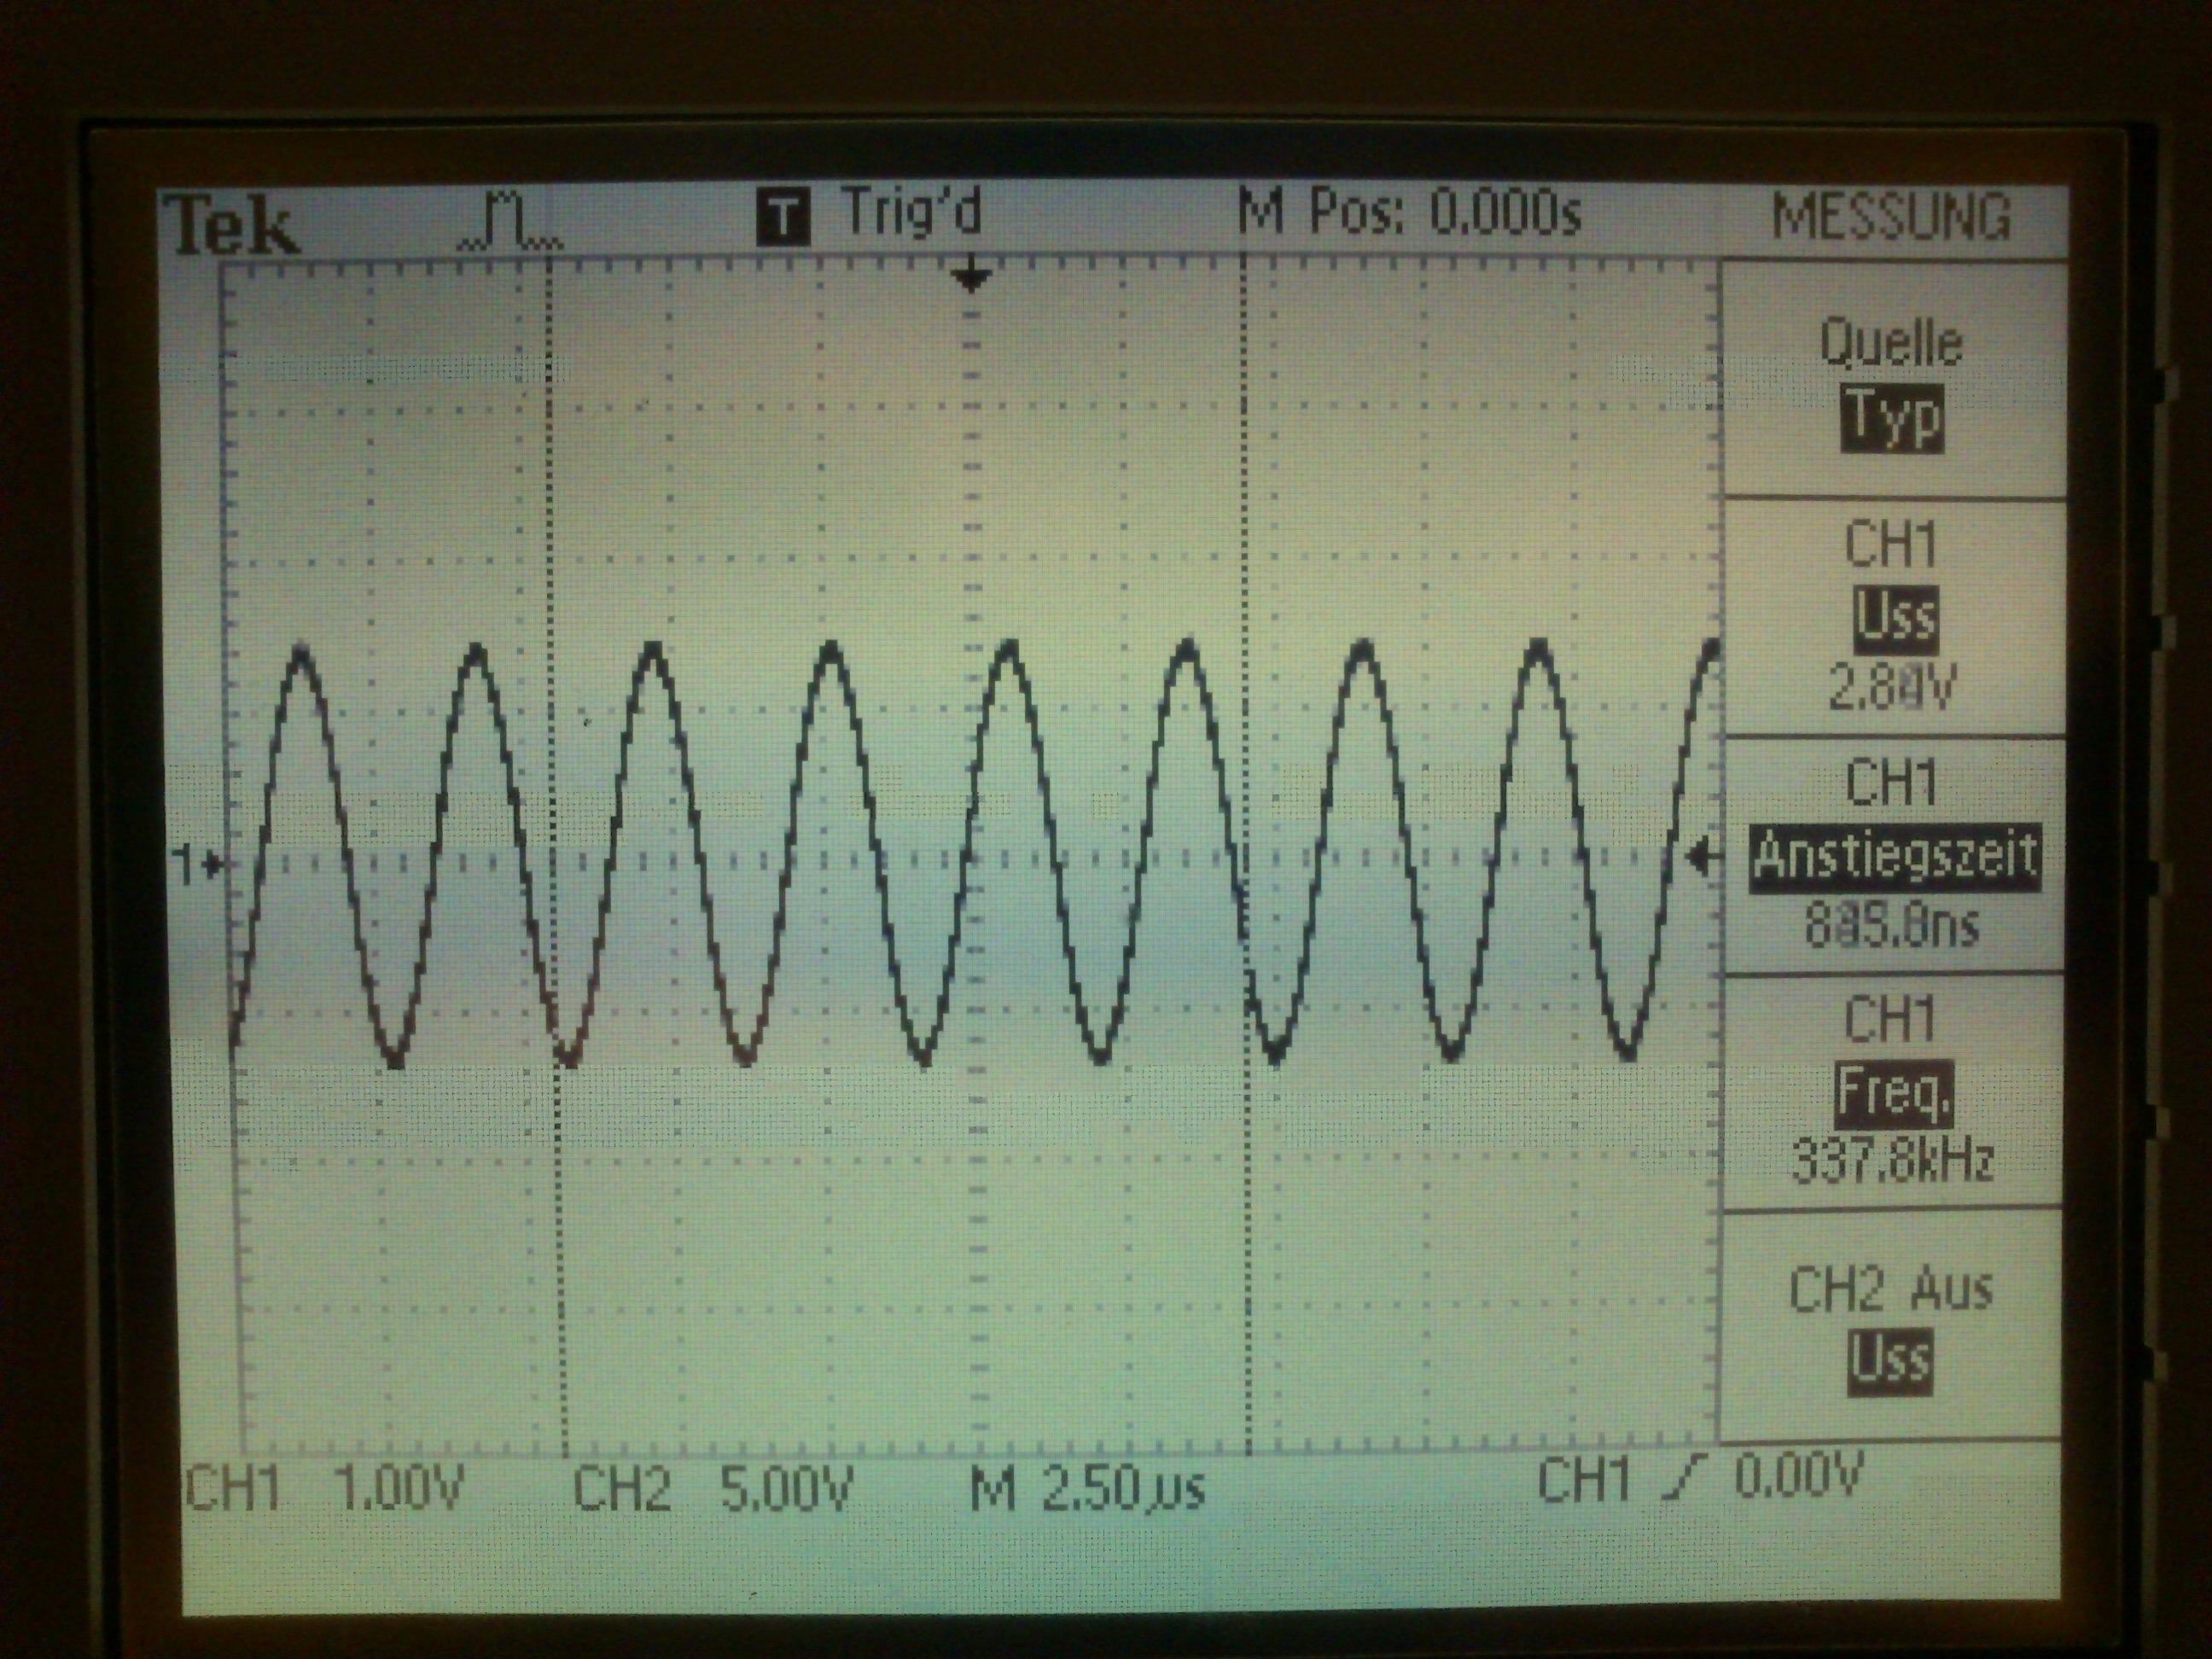
\includegraphics[width=\linewidth]{versuch4/oszi/DSC_0323.JPG}
	\caption{Bestimmung der Grenzfrequenz}
\end{figure}
Ich weiß nicht, wie ich mit den gegebenen Daten eine Aussage über die Eigenschaften des Kabels machen kann.
%%Für die am Oszilloskop gemessene Spannung gilt also:\\
%%
%%$ U_L=U_0\frac{Z_L}{Z_i+Z_L} $ mit $U_0=4V, \; U_L=4V/\sqrt(2)=2.83V,\; Z_i = R_i = 10k\Ohm $ (Da $Z_i$ rein reell ist)\\
%%$\Rightarrow Z_L = \frac{U_L*R_i}{U_0-U_L}=\frac{2.83V*10k\Ohm}{4V-2.83V}=2.4142*10^4 $
%%
%%
%%Bei einem zulässigen Fehler von 5\% bei einem Innenwiderstand von 5k\Ohm darf die Impedanz des Kabels nur 5\% von 5k\Ohm, also 5000\Ohm*0.05=250\Ohm betragen. Aus der eben gemessenen Frequenz lässt sich nun die Frequenz berechnen, ab der die Messung mit Laborstrippen einen zu großen Fehler liefert:\\
%%Aus der Vorlesung ist folgende Formel bekannt: $ Z(f, C) = \frac{1}{2*\pi*f*C}$ \\
%%In unserem Fall gilt: $ Z(340 kHz, C) = \frac{1}{2*pi*340 kHz * C}$ sowie $4V/\sqrt(2)$\\
%%

\subsubsection{Anstiegszeit}
\begin{figure}[H]
	\centering
	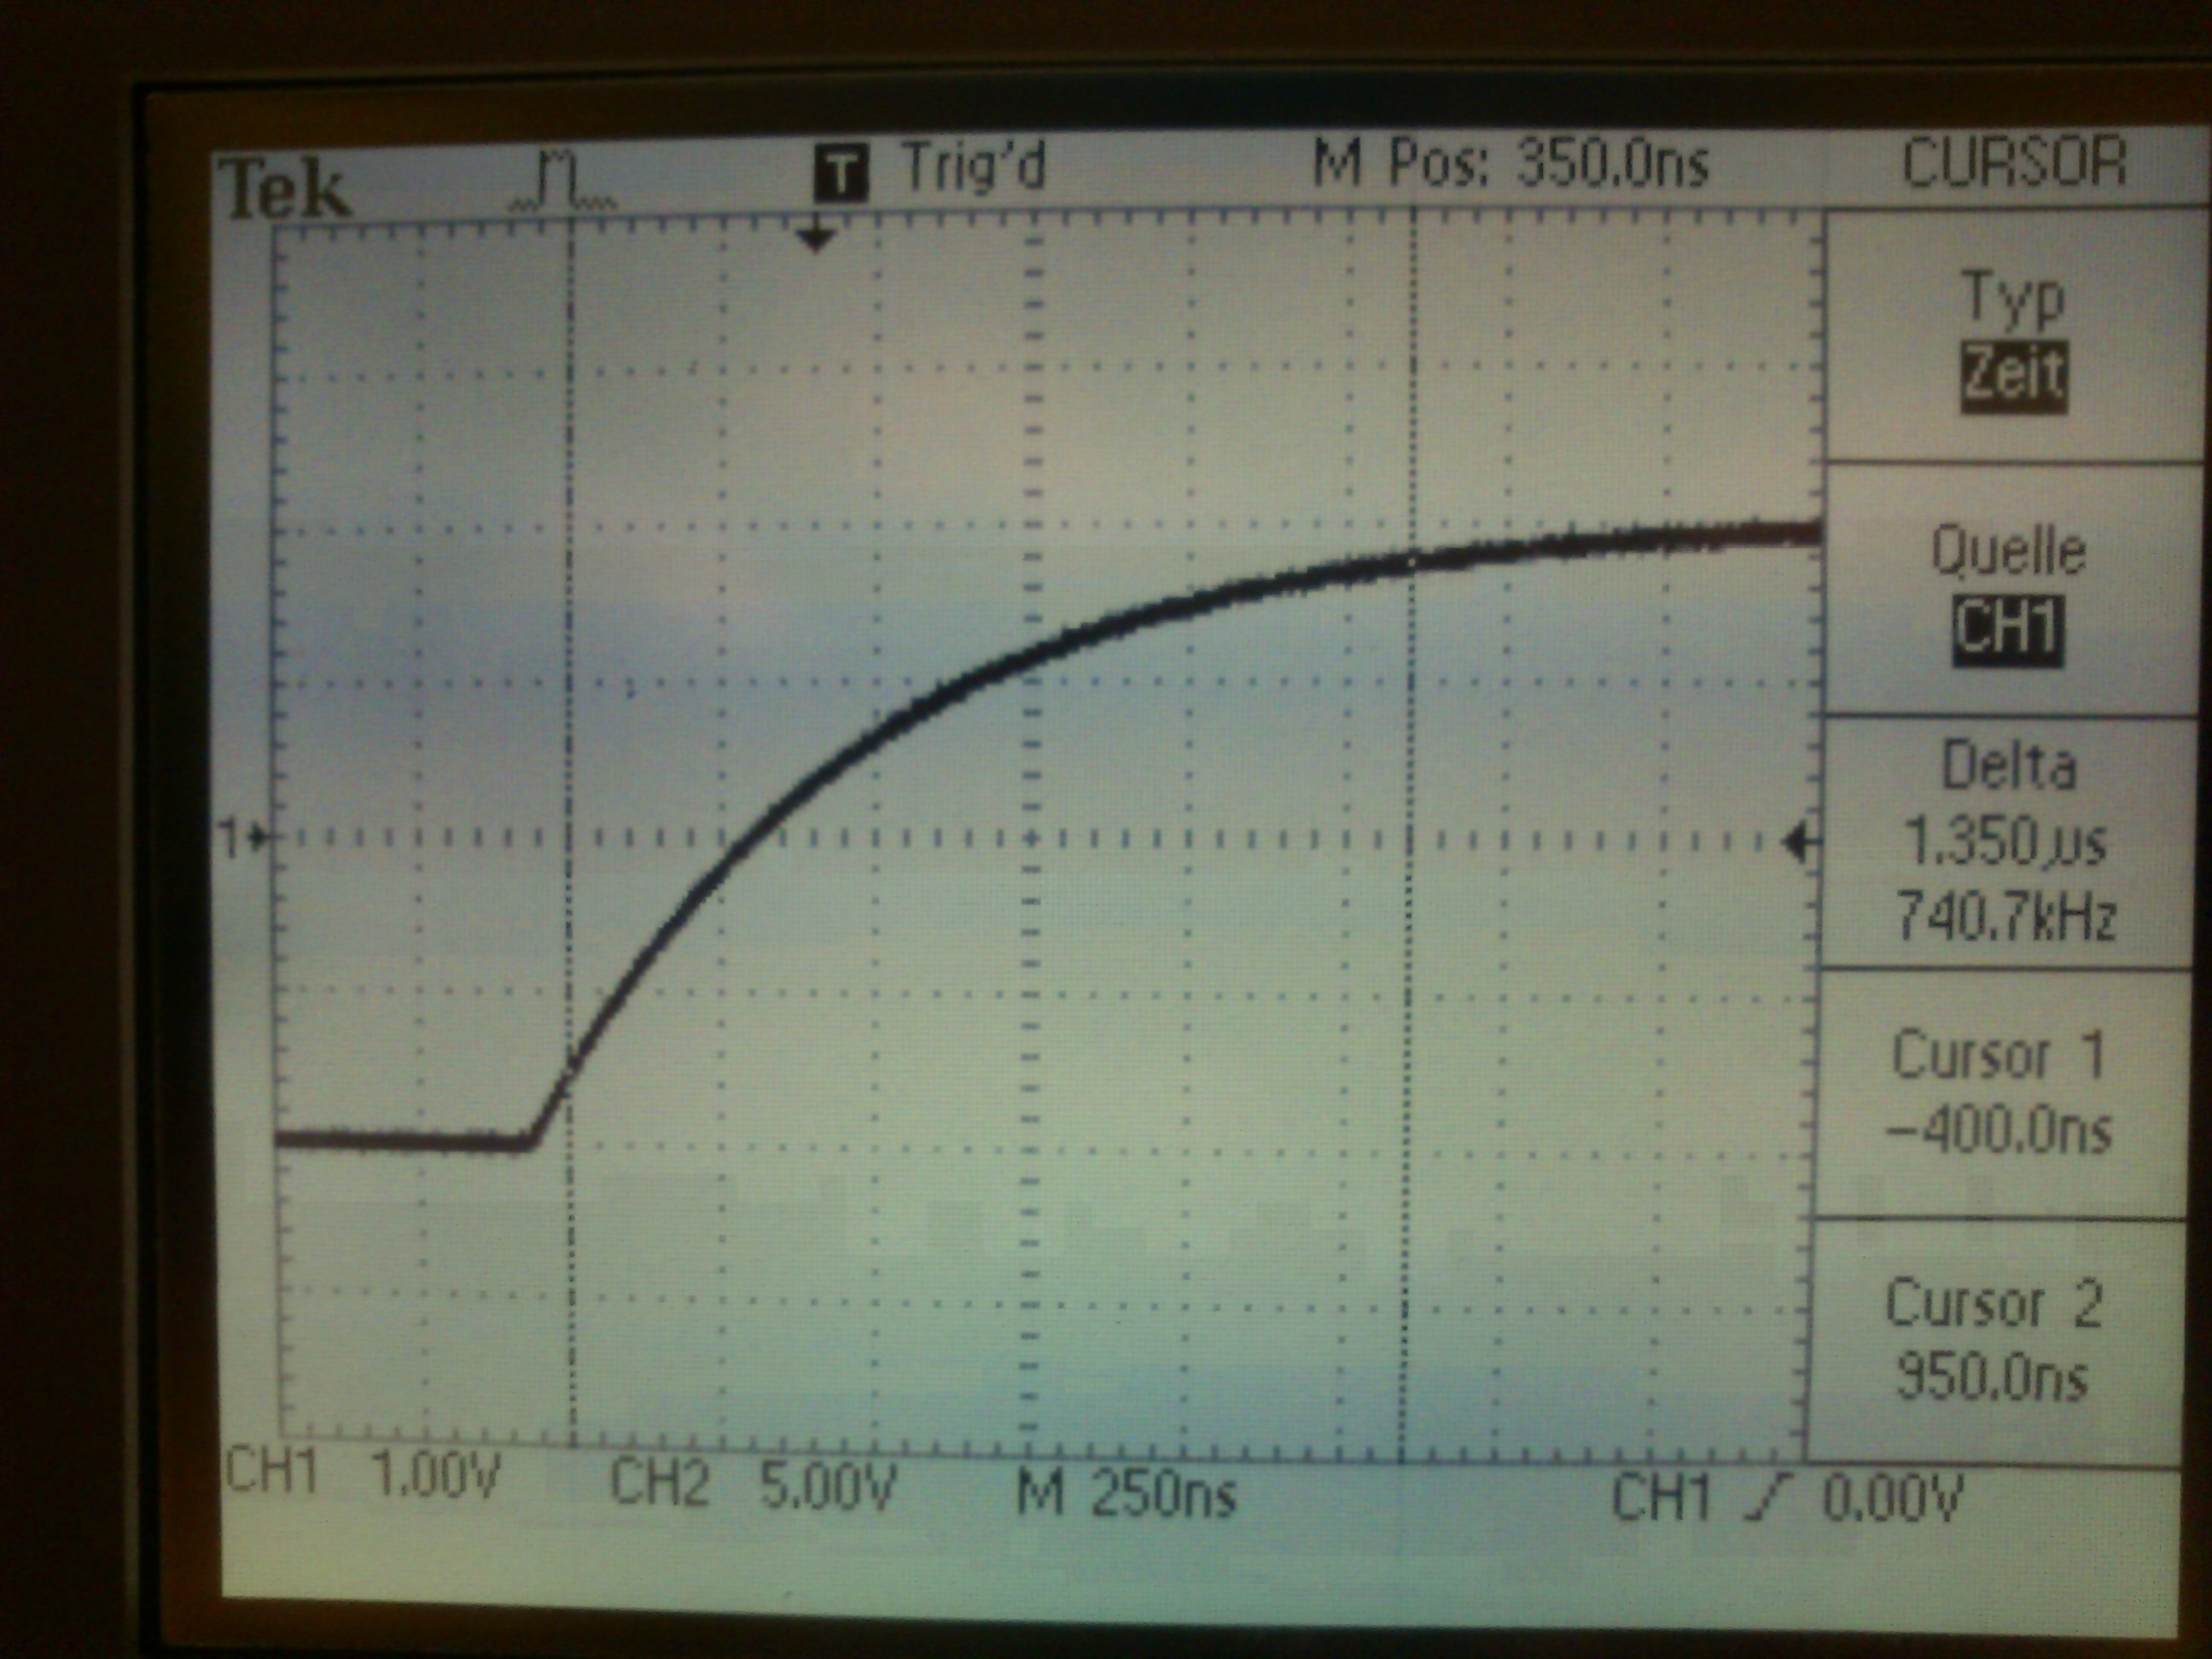
\includegraphics[width=\linewidth]{versuch4/oszi/DSC_0324.JPG}
	\caption{Bestimmung der Anstiegszeit mit Laborstrippe}
\end{figure}
Die Anstiegszeit beträgt 1.350 µs. Der Signalverlauf lässt sich über die Tiefpasscharakteristik des Kabels erklären:
\begin{figure}[H]
	\centering
	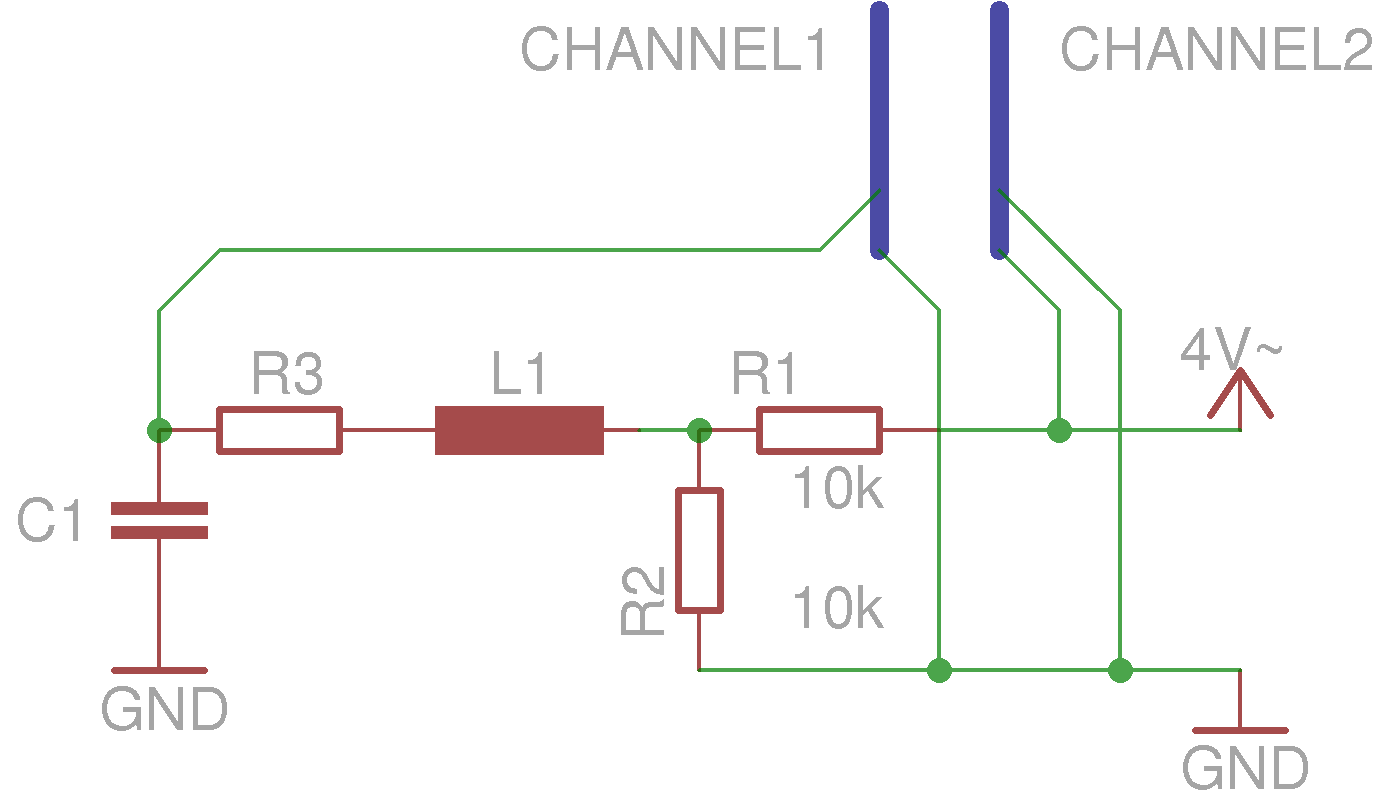
\includegraphics[width=\linewidth]{versuch4/ersatzschaltbild_4_1_b.png}
	\caption{Ersatzschaltbild der Laborstrippe}
\end{figure}
Die Zeitkonstante beträgt dem Hinweis zufolge: $T=\frac{t_2 - t_1}{2,2}=\frac{t_r}{2,2}=\frac{1.35 \mu S}{2,2}=6,1364*10^{-7}$
Daraus könnte man mit $ T=RC \; \Rightarrow C=\frac{T}{R} $ die die Kapazität des Kabels bestimmen, wenn man R kennen würde. Leider ist dem nicht so.

\subsection{Tastköpfe}
\subsubsection*{Frequenzkompensation}
Damit die Frequenz exakt kompensiert wird, müssen die beiden Spannungsteiler den gleichen Teilungsfaktor besitzen:\\
Es muss also $R_1 * C_1 = R2 * (C_K + \frac{C_2*C_{comp}}{C2+C_{comp}})$ gelten.\\
$\Rightarrow \frac{R_1*C_1}{R_2}-C_K=\frac{1}{\frac{1}{C_2}+\frac{1}{C_{comp}}}$
$\Rightarrow \frac{1}{C_2}+\frac{1}{C_{comp}}=\frac{1}{\frac{R_1*C_1}{R_2}-C_K}$\\
$\Rightarrow C_{comp}=\frac{1}{\frac{1}{\frac{R_1*C_1}{R_2}-C_K}+\frac{1}{C_2}}$
$ C_1=15pF, C_2=20pF, R_1=9M\Ohm, R_2=1M\Ohm \Rightarrow C_{comp} = 20pF$\\
Wenn man einen normalen Schraubenzieher zum Einstellen verwendet, kann er die Einstellung mit seiner eigenen Kapazität beeinflussen.\\
Statt nur der Bandbreite ist es sinnvoll anzugeben, bis zu welcher Frequenz Signale unverzerrt dargestellt werden können, also den Frequenzgang.
\subsubsection{Anstiegszeit}
Die Anstiegszeit wurde mit dem Tastkopf zu 180 ns ermittelt, die Anstiegszeit mit Laborstrippe ist als 7,5 mal so groß.
\begin{figure}[H]
	\centering
	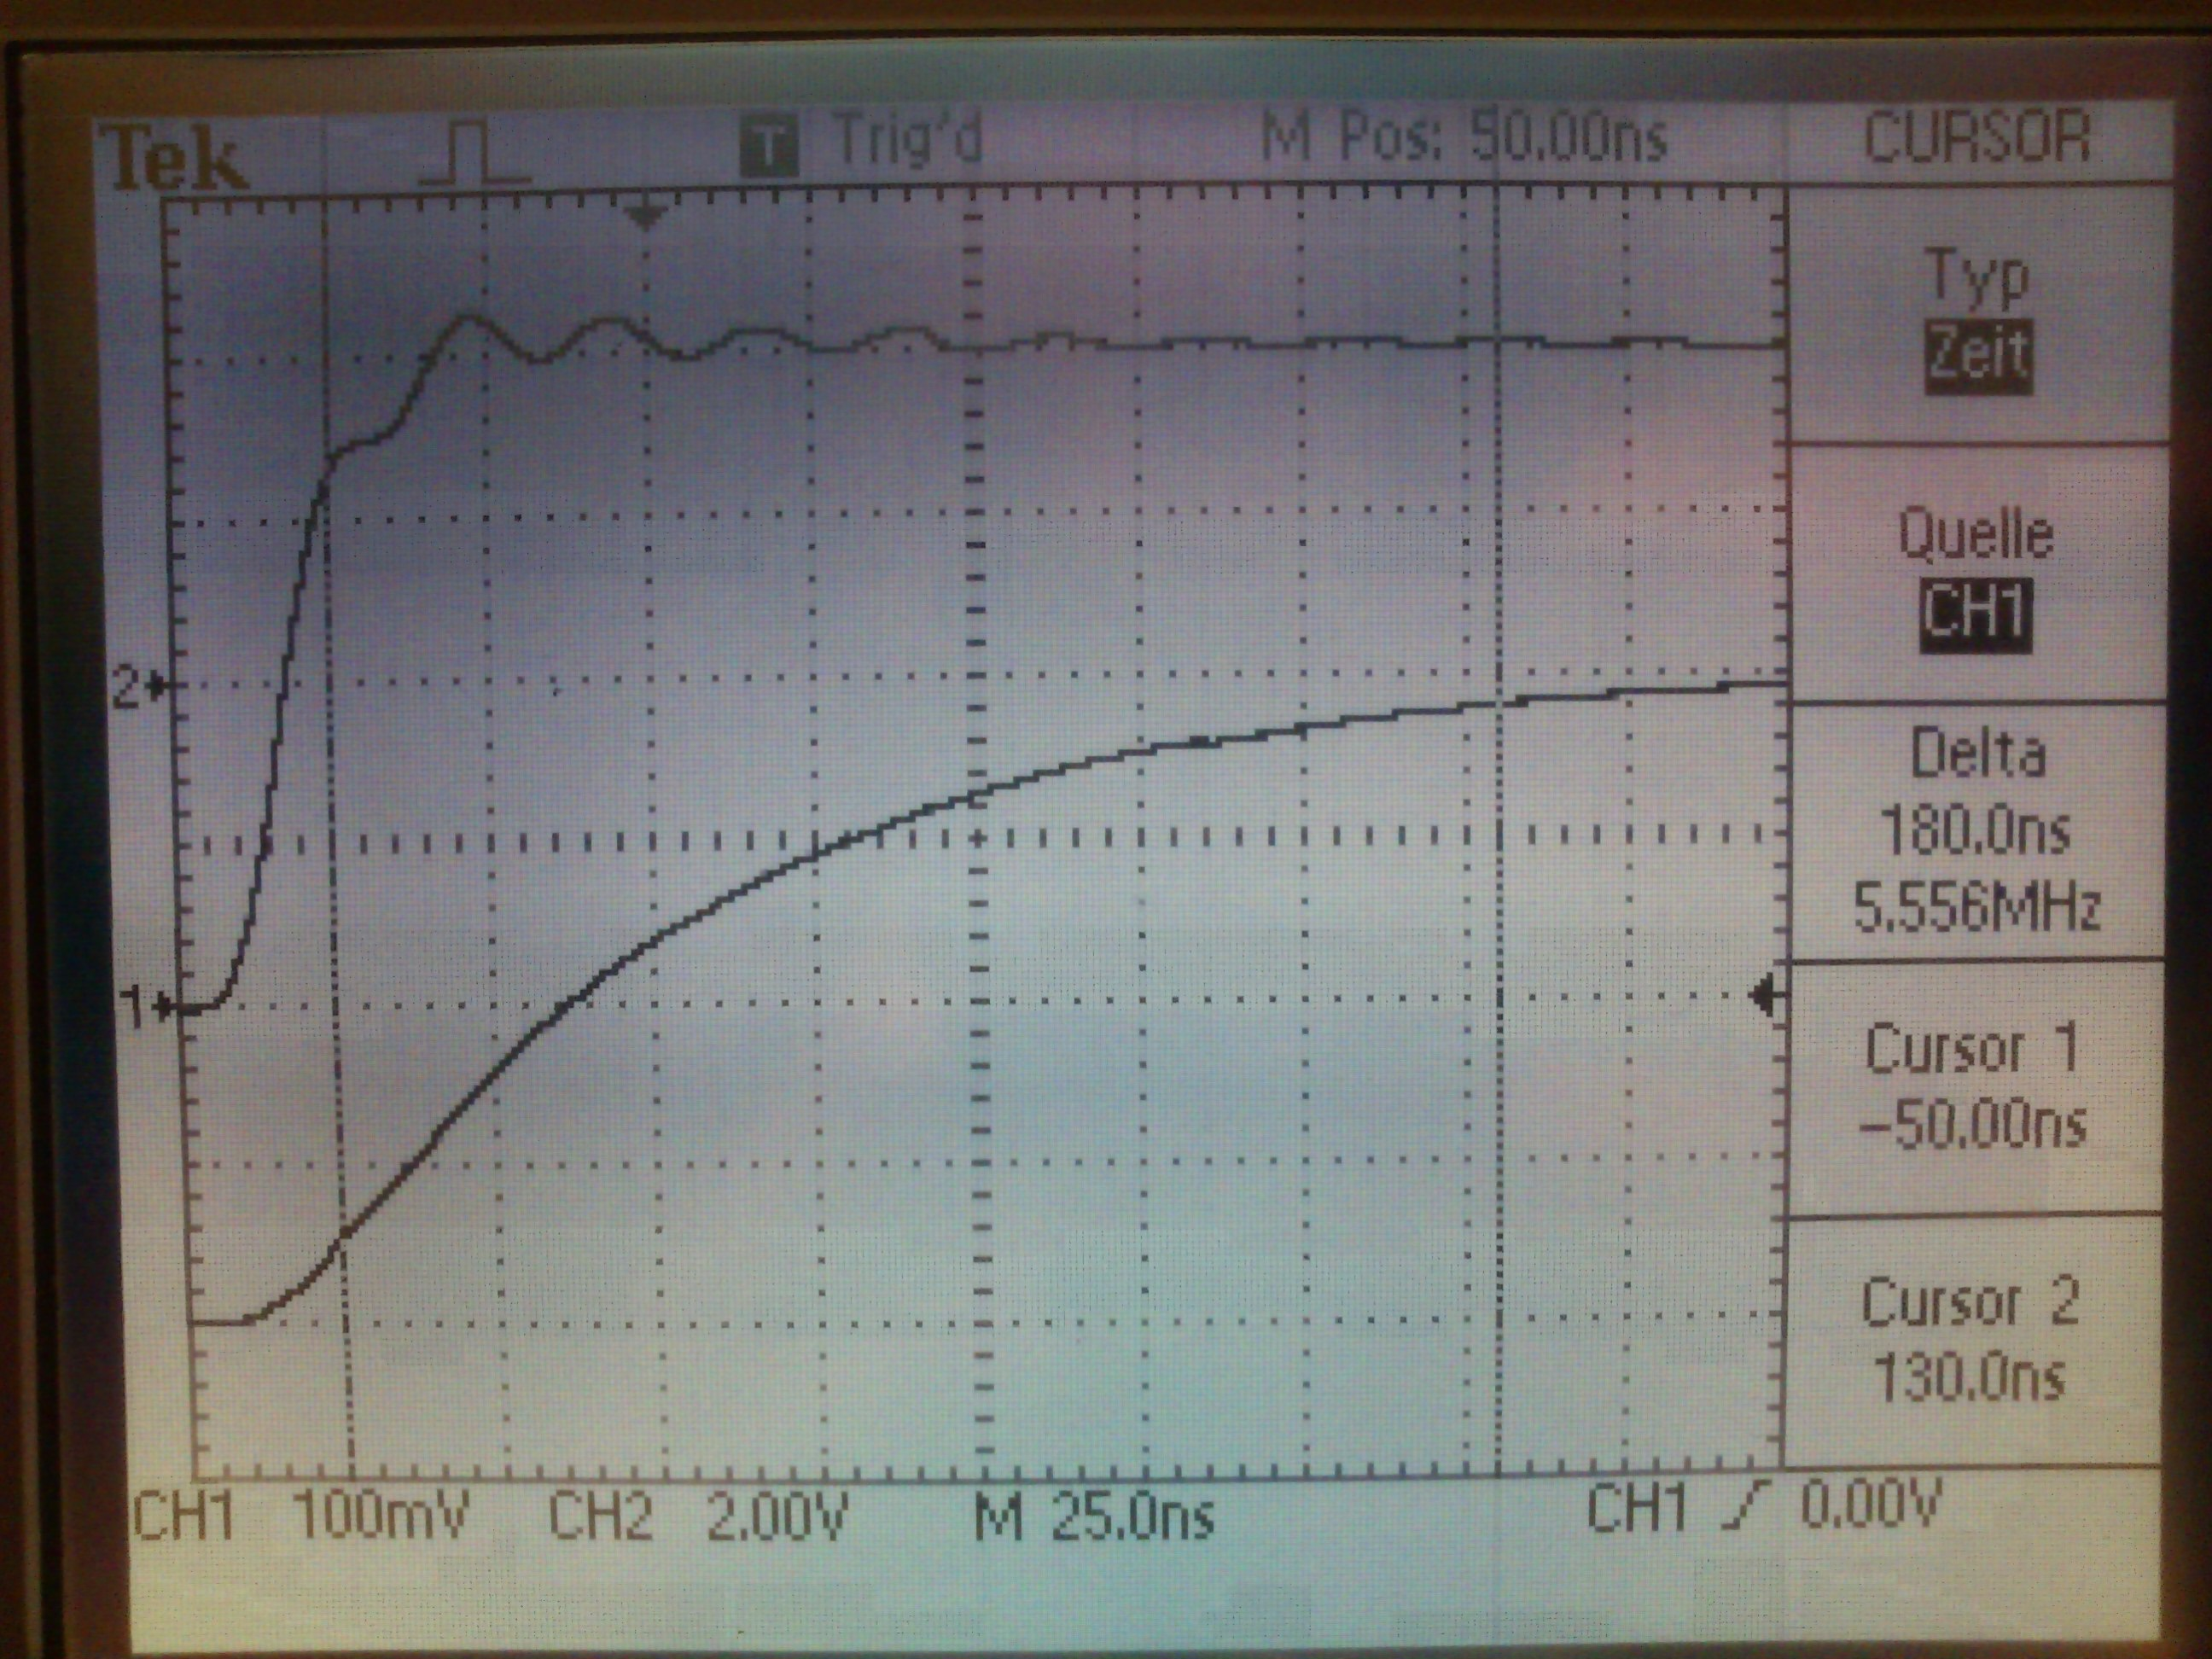
\includegraphics[width=\linewidth]{versuch4/oszi/DSC_0335.JPG}
	\caption{Bestimmung der Anstiegszeit mit Tastkopf}
\end{figure}

Damit lässt sich die Kapazitive Belastung der Spannungsquelle berechnen. Wir wissen, dass der Innenwiderstand der Spannungsquelle 5kOhm ist, somit folgt für die kapazitive Belastung:\\
$ T=180ns=R*C, \; R=5k\Ohm \; \Rightarrow \; C=\frac{T}{R}=\frac{180ns}{5k\Ohm}=36pF$

\subsubsection{Bezugspotential}
\begin{figure}[H]
	\centering
	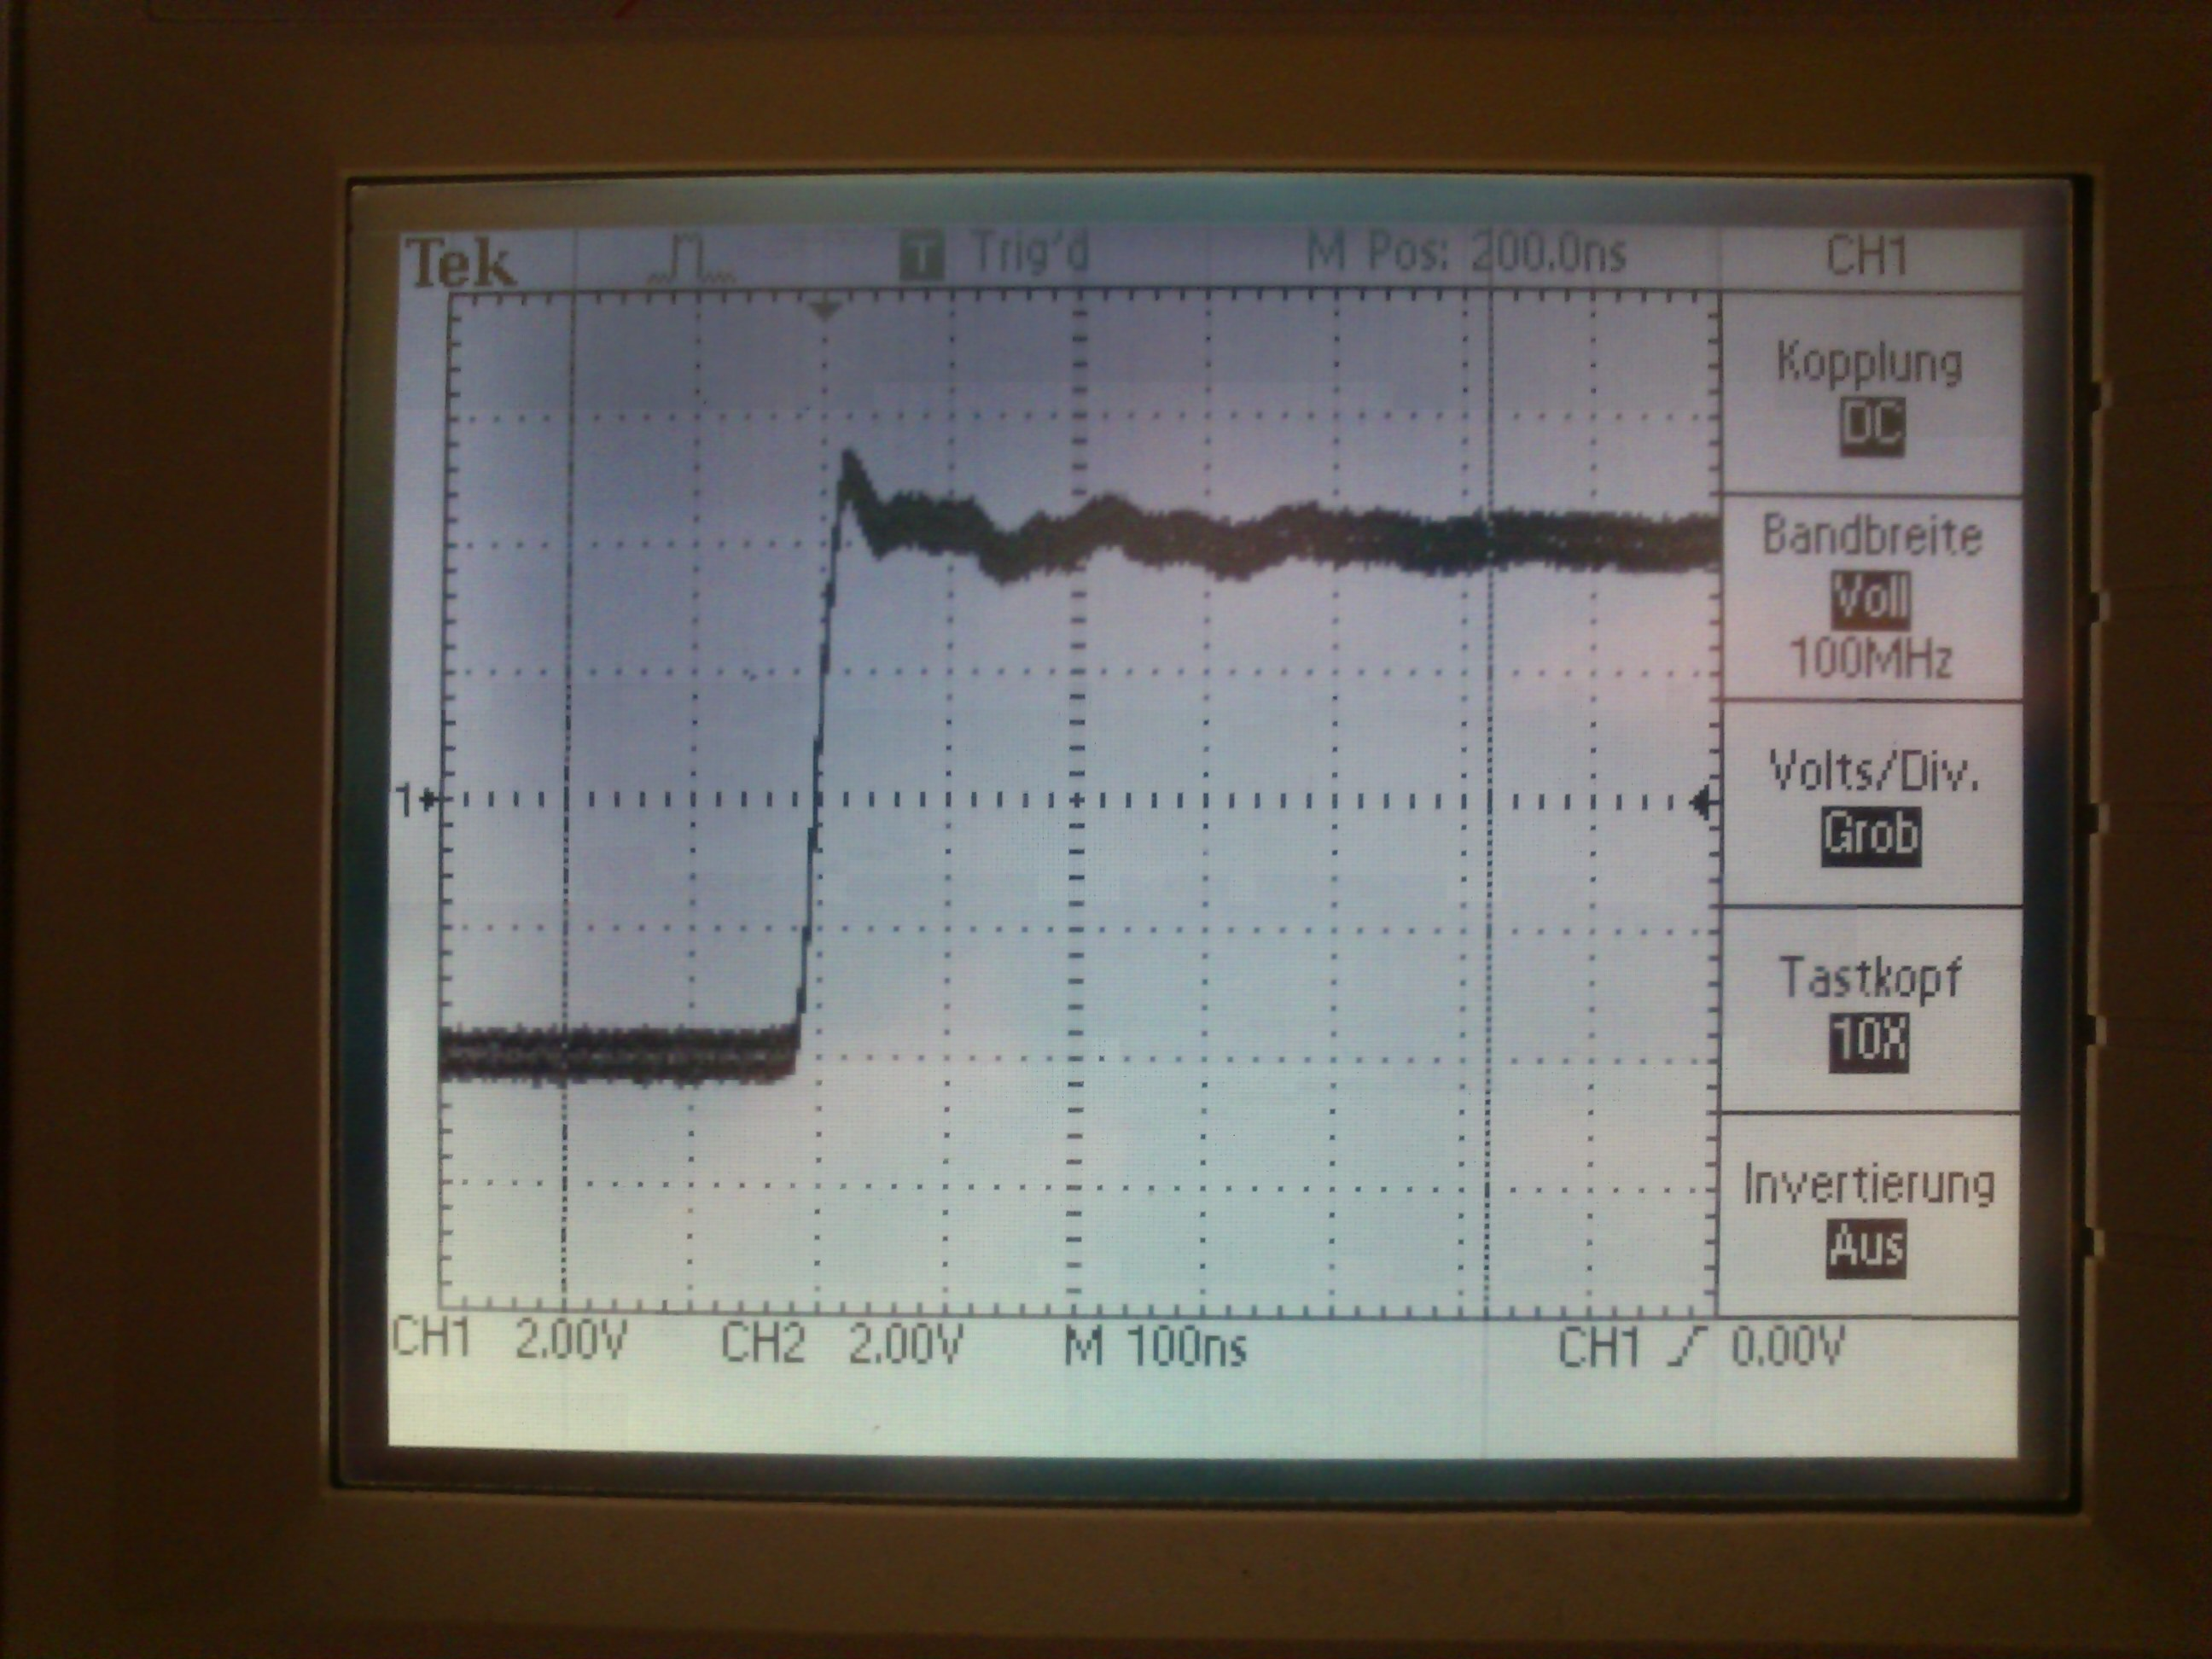
\includegraphics[width=\linewidth]{versuch4/oszi/DSC_0340.JPG}
	\caption{Einschwingvorgang bei offener Masseverbindung (grob)}
\end{figure}

\begin{figure}[H]
	\centering
	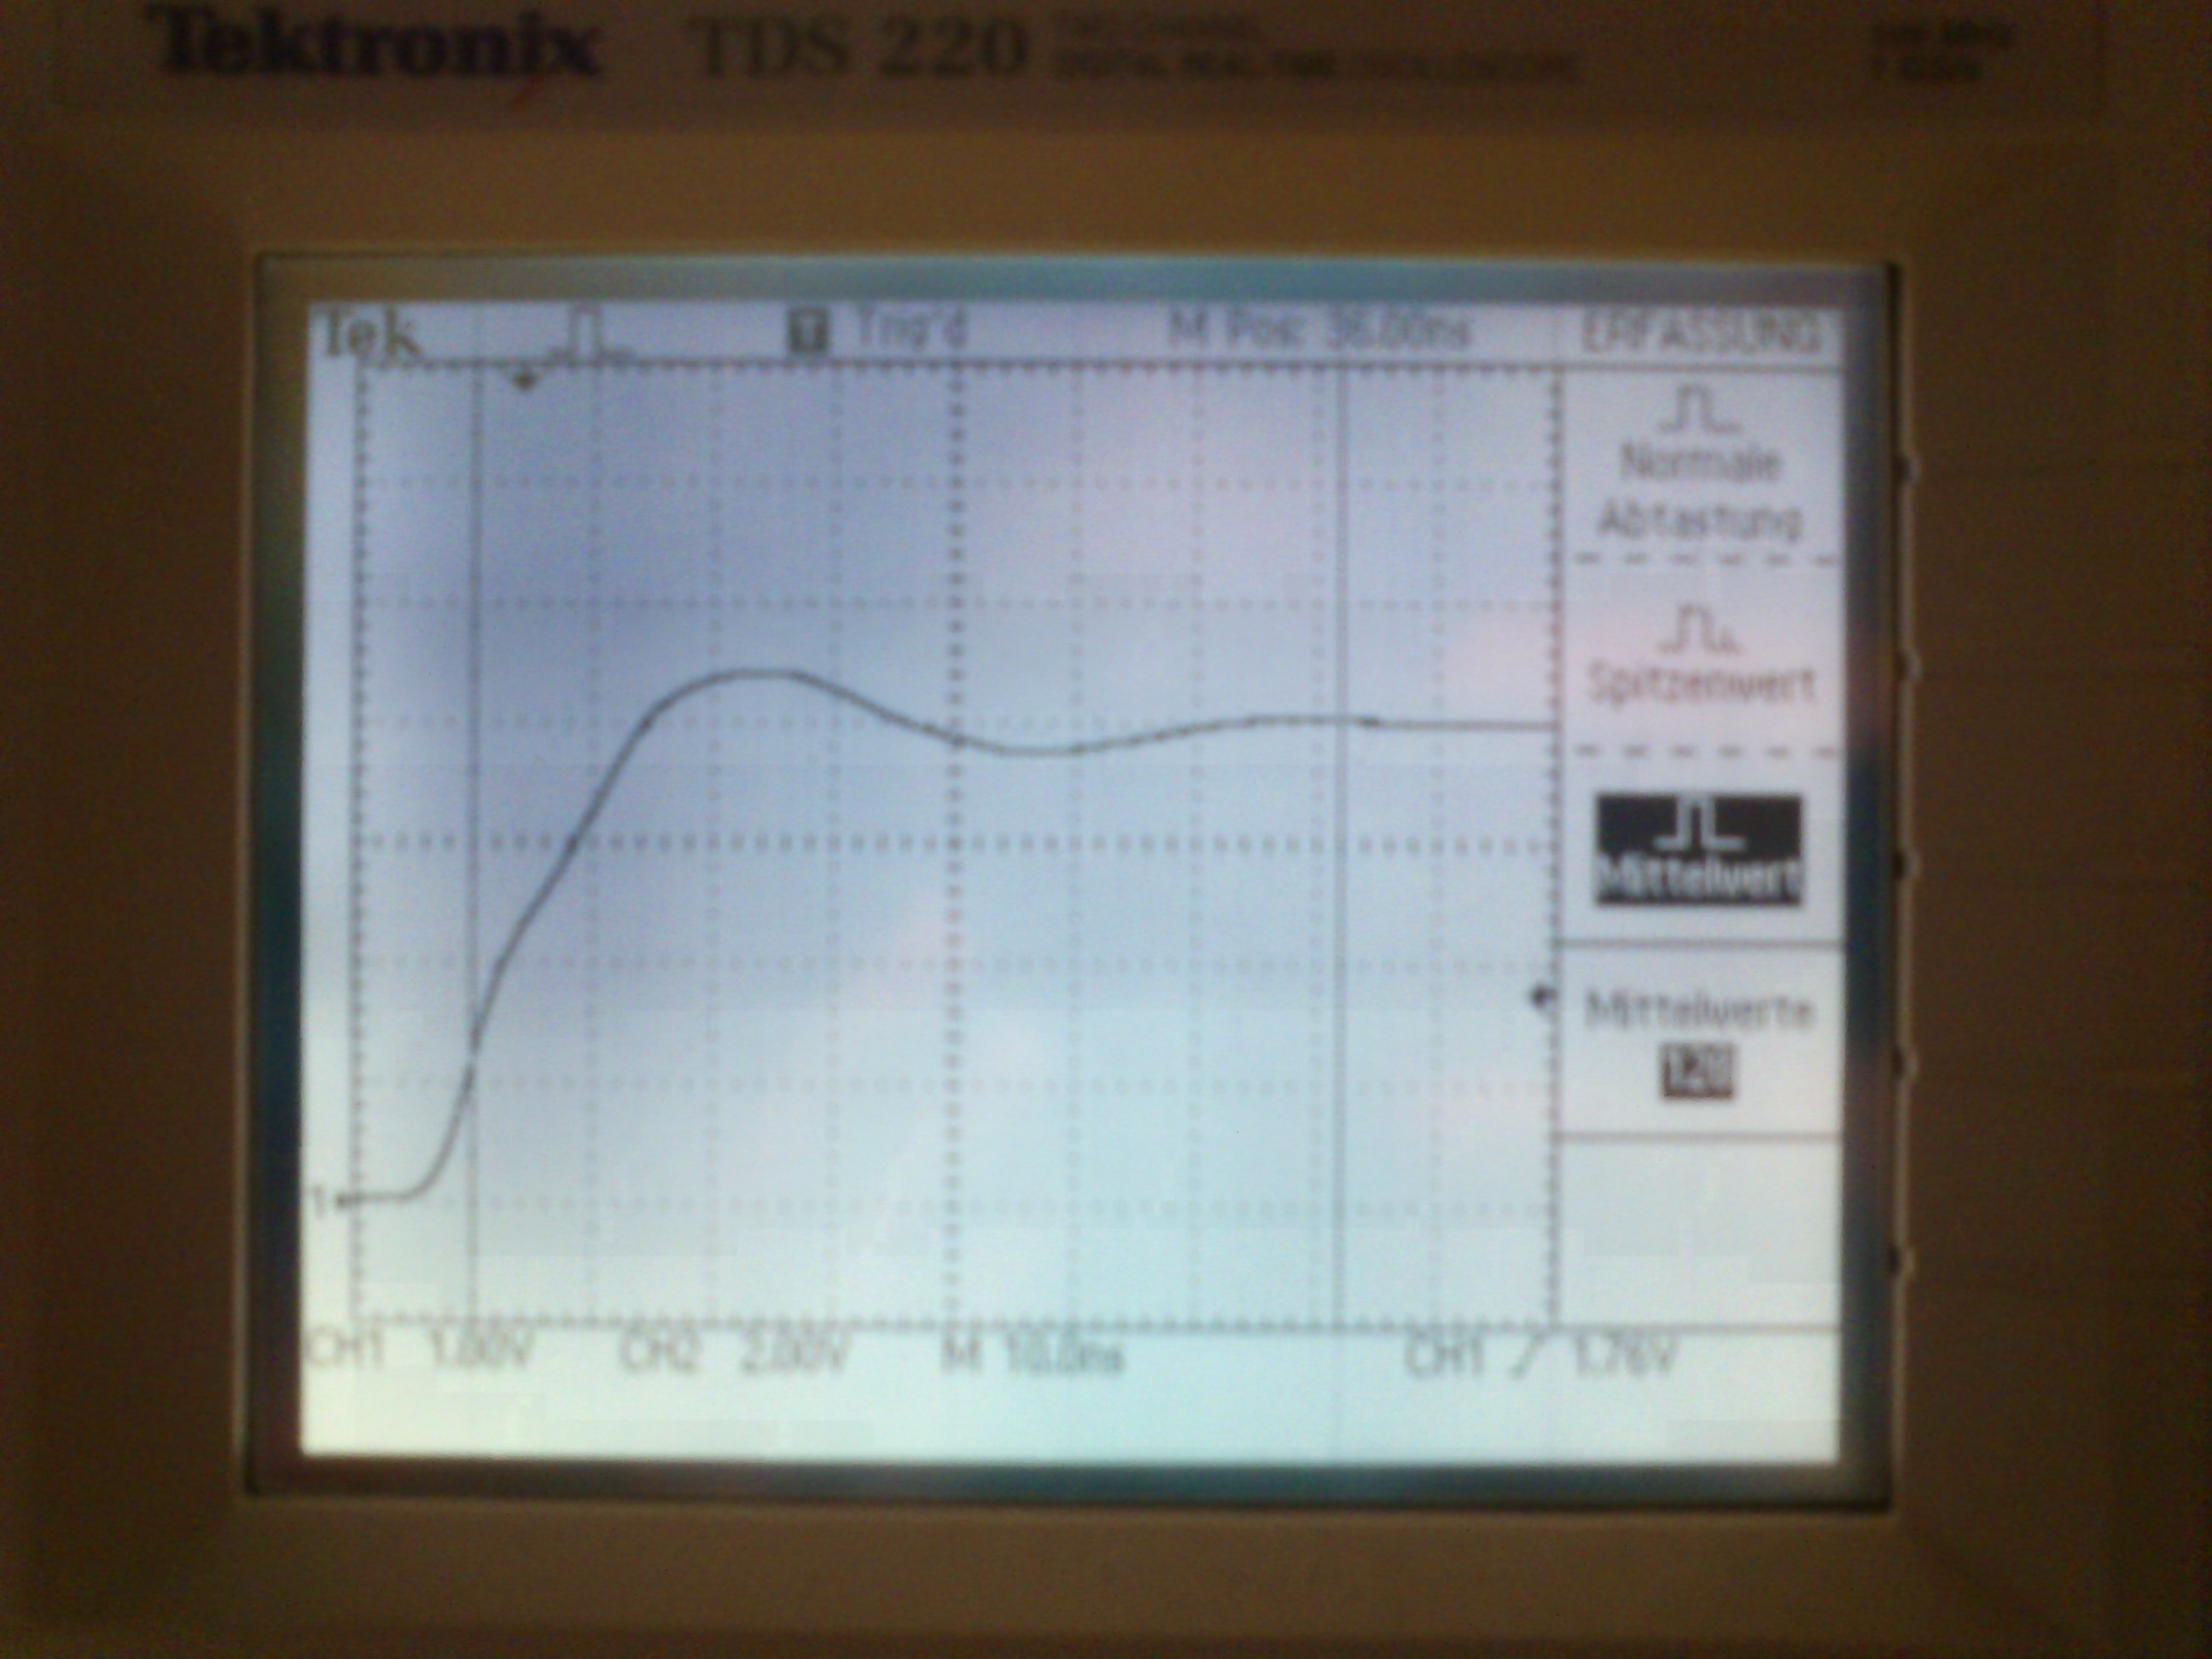
\includegraphics[width=\linewidth]{versuch4/oszi/DSC_0342.JPG}
	\caption{Einschwingvorgang bei offener Masseverbindung (fein)}
\end{figure}
Wie man erkennt, ist die Schwingung stakr gedämpft und nach einer Periode praktisch nicht mehr erkennbar. Als Werte für die Einhüllende bleiben somit eigentlich nur (0ns, 0.5V), (20ns, 0.25V) und (45ns, 0.10V). Mit dem Ansatz aus der Anleitung folgt somit:\\
$U_0=U(t=0)=0.5V;\; U(20ns)=U_0*e^(T*30ns)=0.25V\; \Rightarrow T=-\frac{ln(0.5V)}{20ns}=0.34657\mu s$\\
Überprüft man dies nun mit dem 3. Wert, so erhält man:\\
$ U(45ns)=U_0*e^{-T*45ns}=0.10511V $. Somit bestätigt sich sich die Berechnung.

Schließt man nun den Masseanschluss auch noch an, so erhält man folgendes Bild:
\begin{figure}[H]
	\centering
	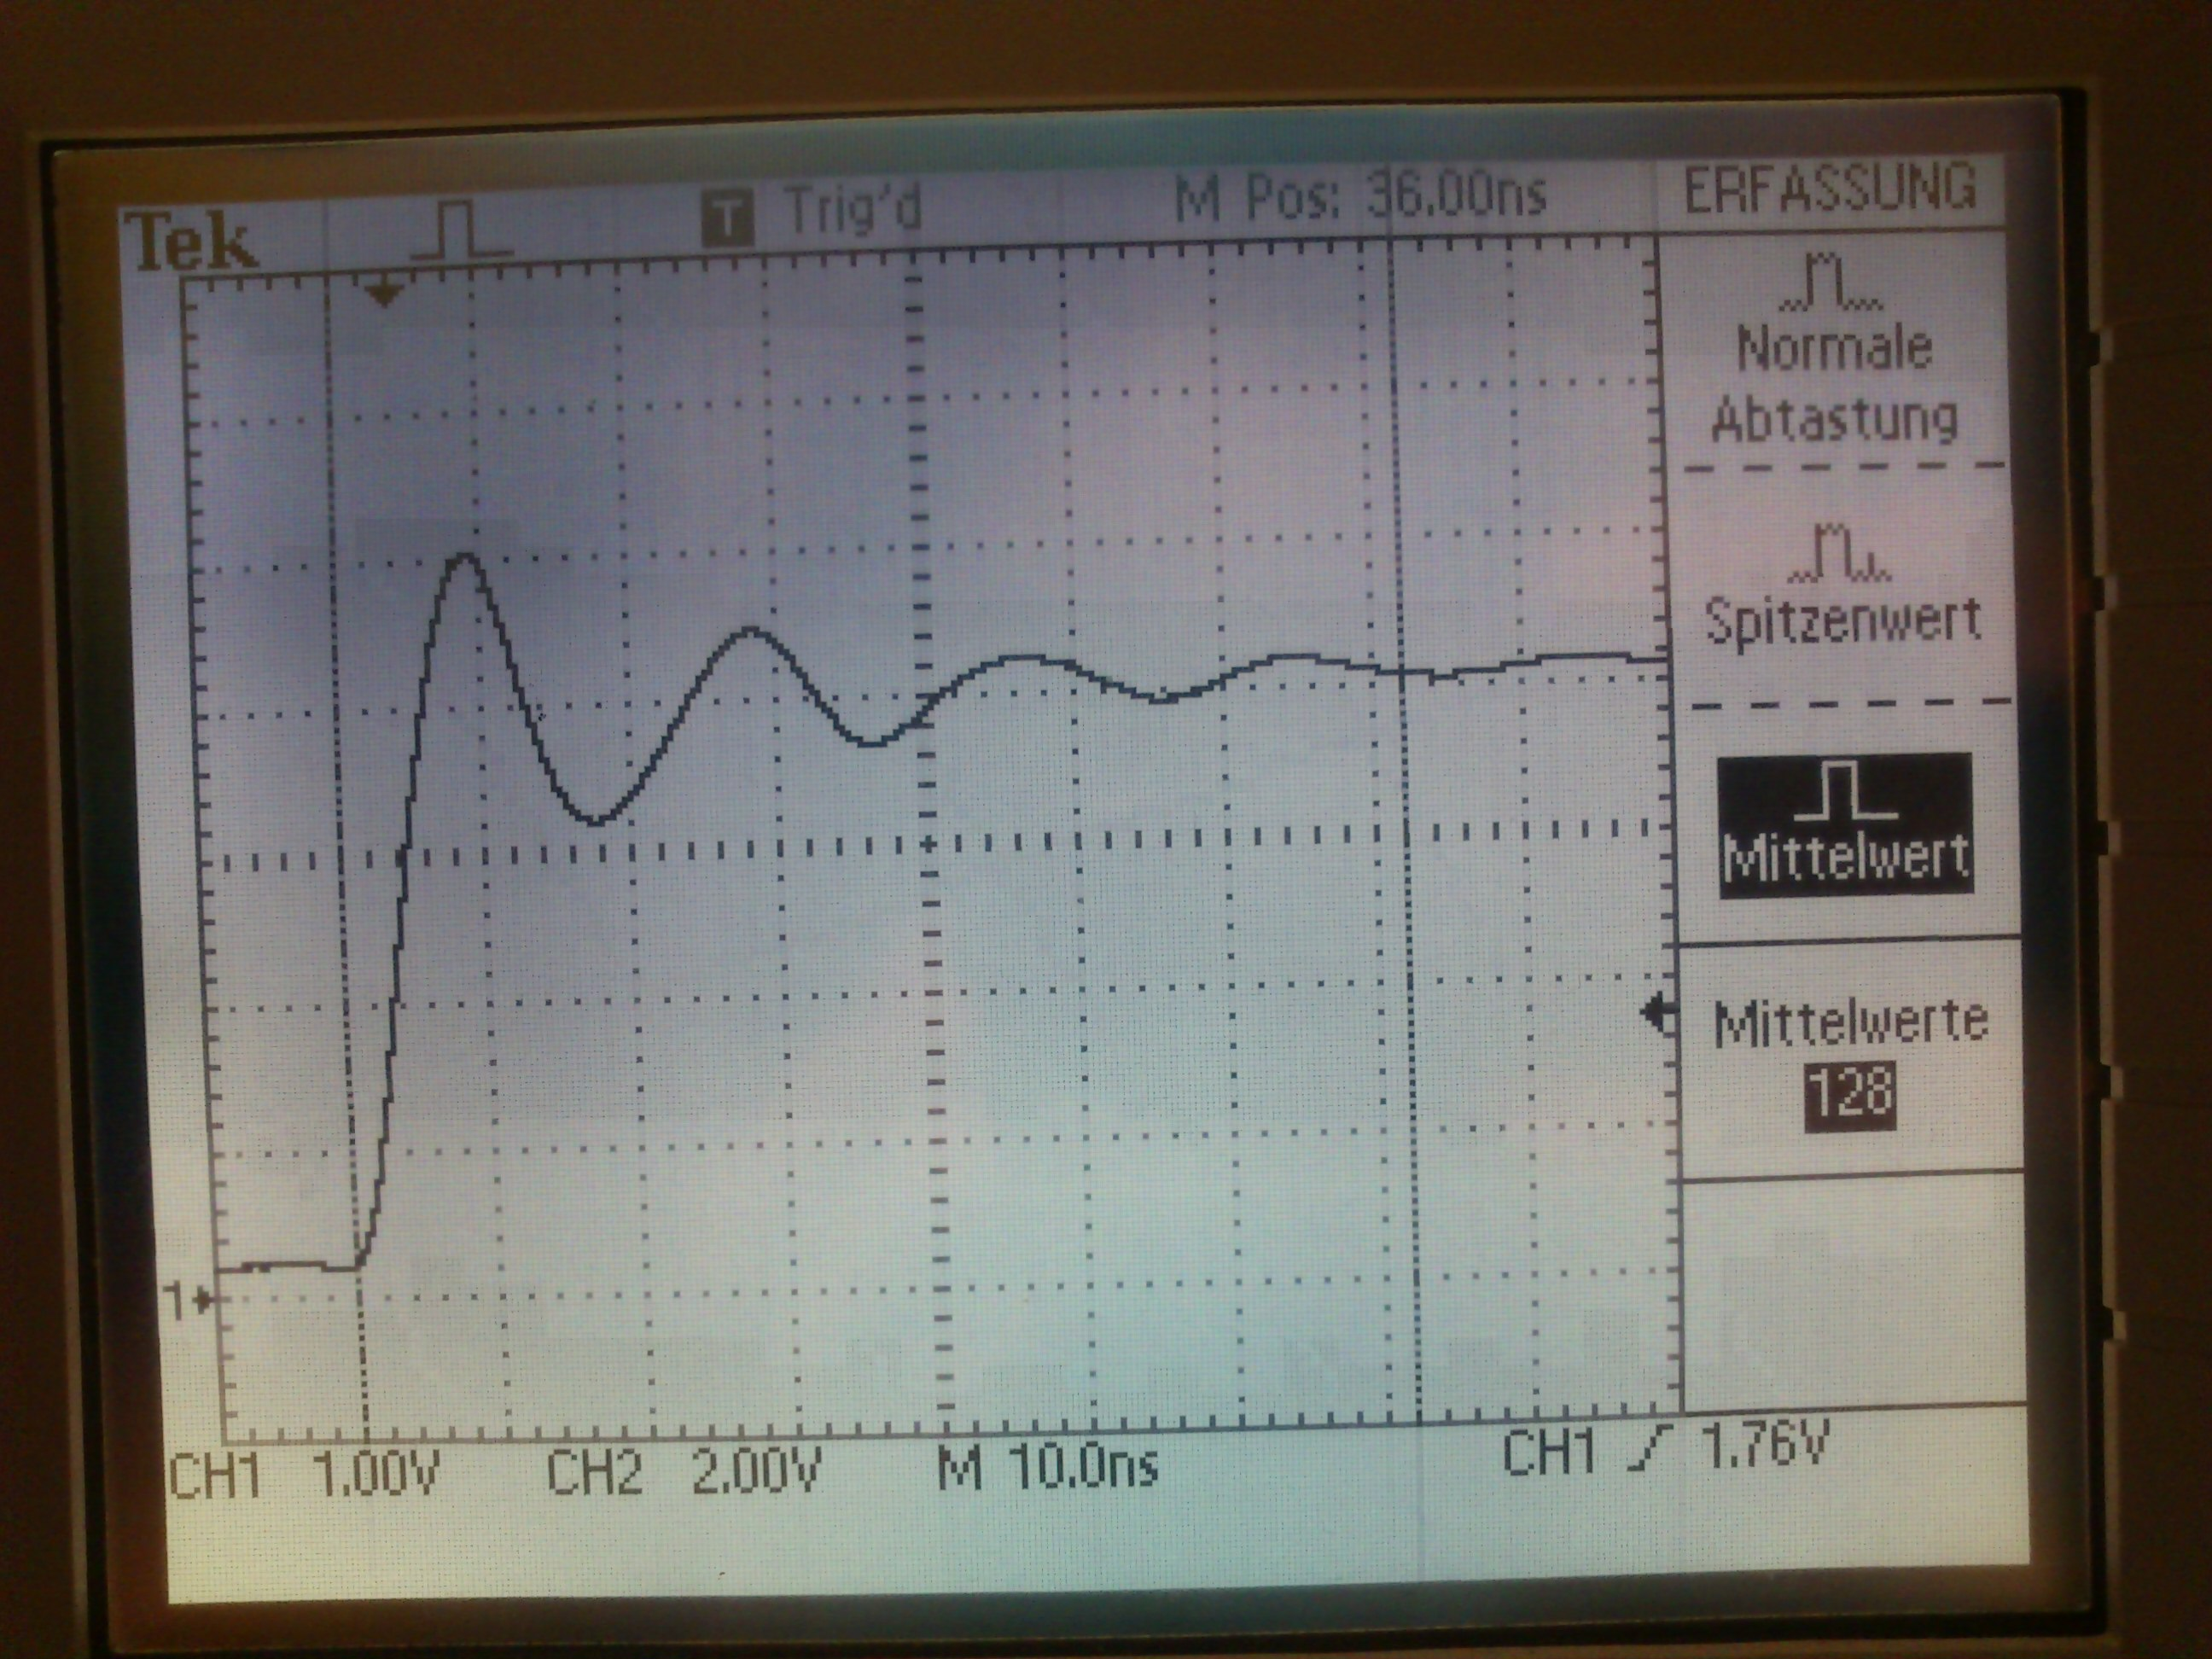
\includegraphics[width=\linewidth]{versuch4/oszi/DSC_0344.JPG}
	\caption{Einschwingvorgang bei geschlossener Masseverbindung}
\end{figure}
Eigentlich hätte ich erwartet, dass nun ein sauberes Rechtecksignal zu sehen sei, insbesondere, da in der Spannungsquelle keine nennenswerten Kapazitäten vorhanden sein sollten.

\subsection{Laufzeitmessung}
In diesem Versuch wurde die Laufzeit in einem Koaxialkabel gemessen.
\begin{figure}[H]
	\centering
	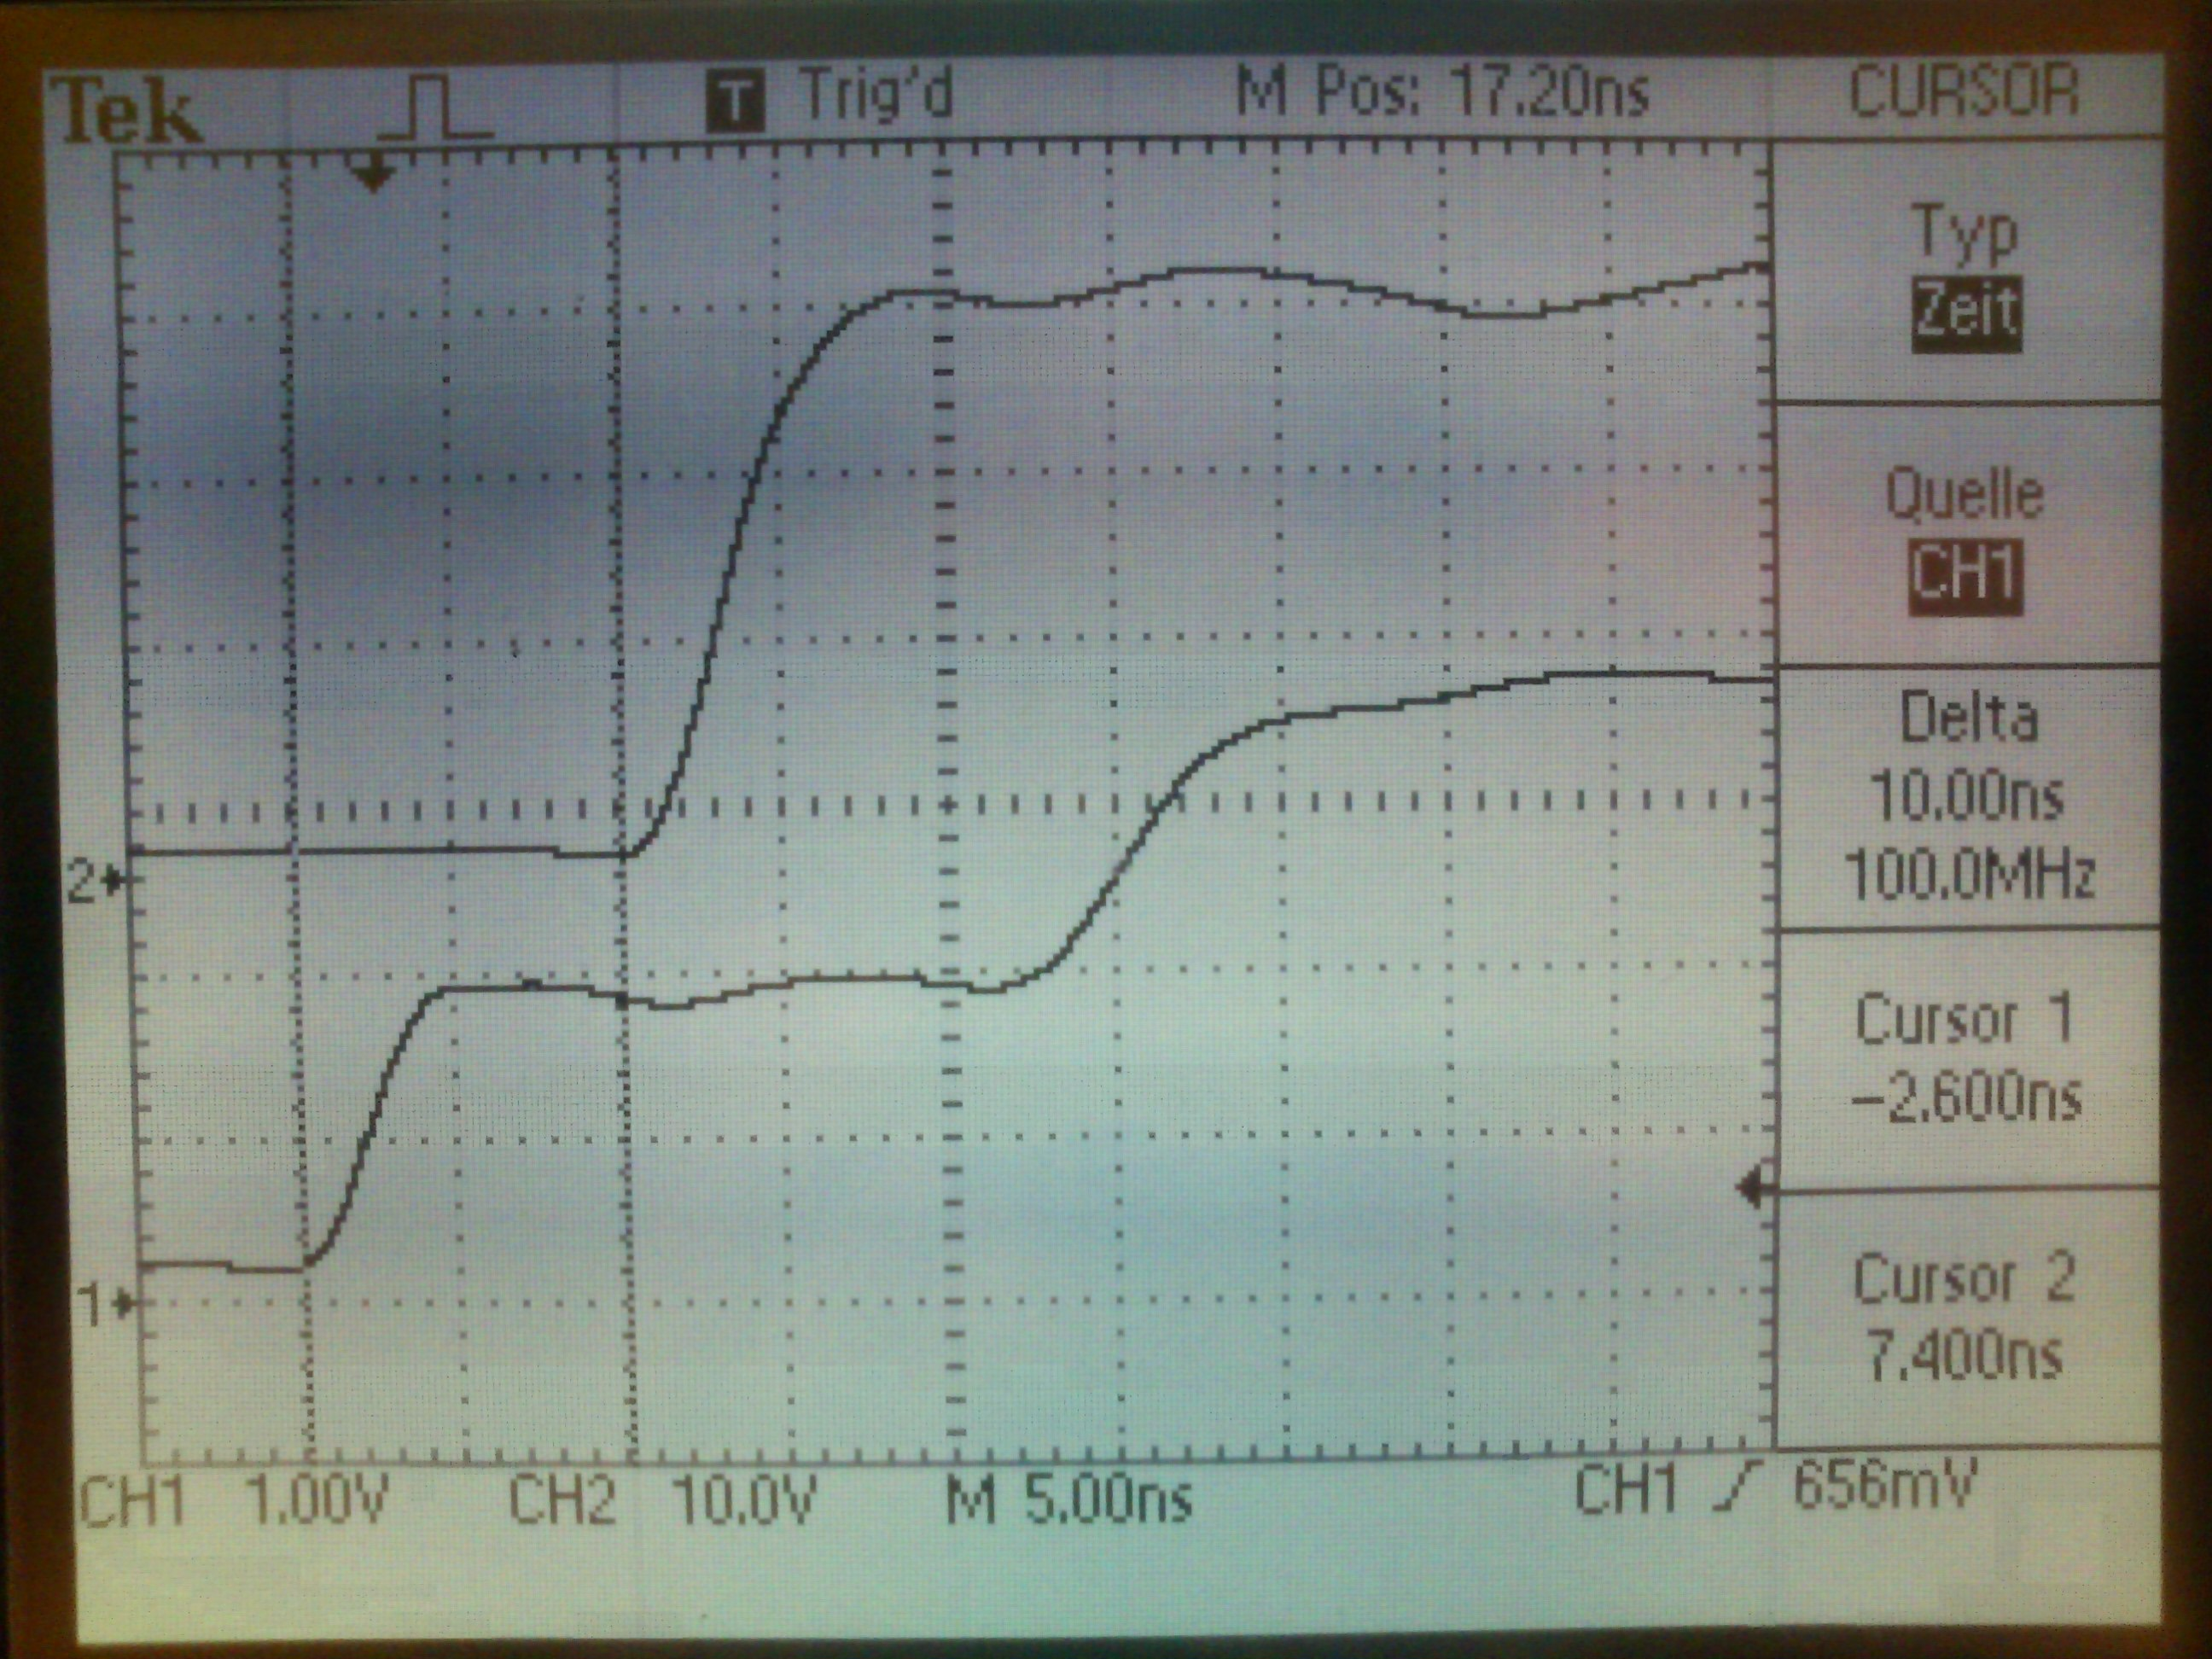
\includegraphics[width=\linewidth]{versuch4/oszi/DSC_0349.JPG}
	\caption{Die Laufzeit beträgt 10ns}
\end{figure}
Für die Dielektrizitätskonstante des Isolators gilt:\\
$ T_L=10ns=\sqrt{\epsilon_r}/c*L;\; c = 3*10^8 \frac{m}{s};\; L=Kabell"ange=2m;$\\
$ \Rightarrow\; \epsilon_r=(\frac{T_L}{L}*c)^2=(\frac{10ns}{2m}*3*10^8)^2=2.25 $\\

Der "`seltsame"' Verlauf auf CH1 kommt von der Reflektion am Ende des 2. Kabels. Steckt man eine 50\Ohm -Terminierung auf, so verschwindet die Reflektion:
\begin{figure}[H]
	\centering
	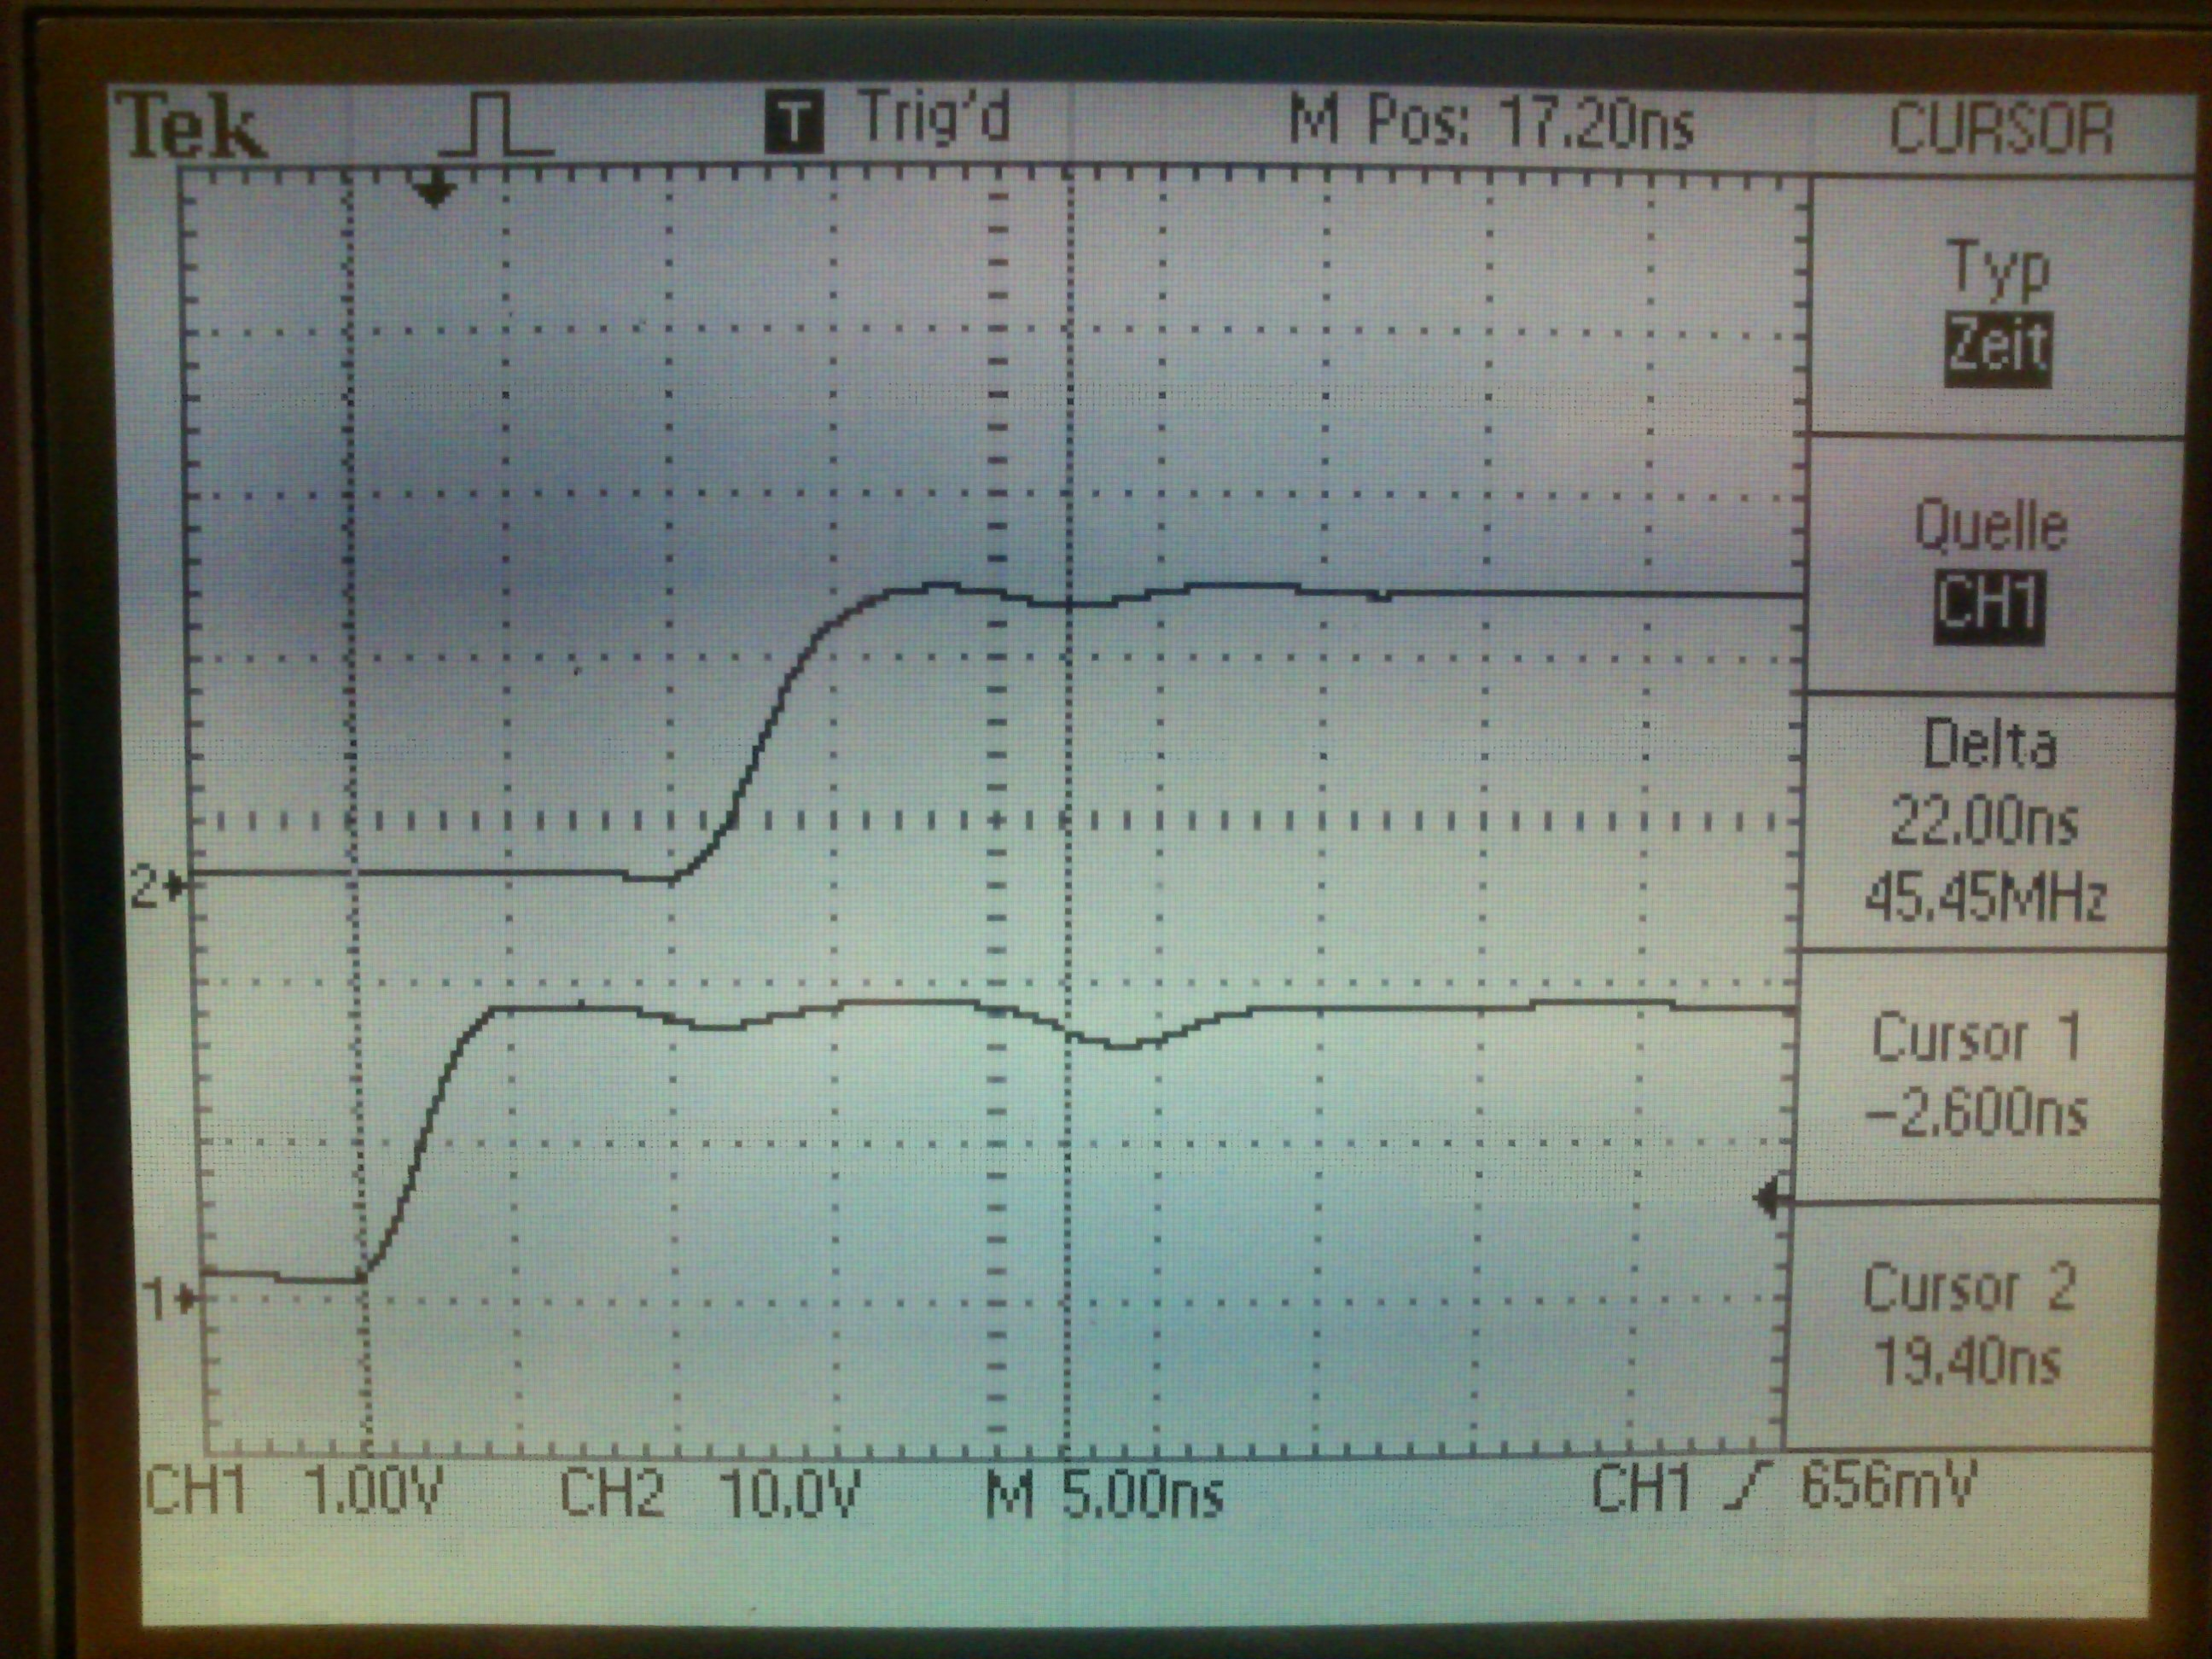
\includegraphics[width=\linewidth]{versuch4/oszi/DSC_0353.JPG}
	\caption{Das Signal mit passender Terminierung}
\end{figure}
Am Signalausgang sind die Effekte auf Grund des geringeren Flankensteilheit nicht mehr sauber zu erkennen.

Ein Kabel sollte Terminiert werden, wenn die Signallaufzeit größer als ein sechstel der Anstiegszeit ist \cite{myc-wellenwiderstand}. Somit genügt es, die Länge zu bestimmen, bei der die Signallaufzeit gerade ein sechstel der Anstiegszeit ist:
$ T_L=10ns=\sqrt{\epsilon_r}/c*L;\; T_L=\frac{1,4ns}{6};\; \epsilon_r=5,5 \Rightarrow L=\frac{T_L*c}{\sqrt{\epsilon_r}}=0.029848m=2,9cm $\\
Somit müsste man bei Kabeln über 3 cm Länge eigentlich eine Terminierung vorsehen. Die Webseite besagt jedoch auch, dass die Terminierung spätestens beim Doppelten bis 3-fachen dieses Wertes nötig sei. Somit käme man immerhin 12- bis 18 cm weit ohne Terminierung.

\subsection{Spektralanalyse}
\subsubsection{Resonanzfrequenz, Bandbreite}
Die Resonanzfrequenz des Schwingkreises beträgt:\\
$ C=1nF=1*10^{-9 F};\; L=0.1mH=1*10^{-4} H;\; f_0=\frac{1}{2*pi*sqrt(LC)} =  503.29kHz $

Das Amplitudenmaximum wurde bei 513kHz zu 13.1V bestimmt, also knapp 10kHz über dem errechneten Wert. 70\% des Maximums sind als 9.17V. Diese treten bei 506kHz und 520kHz auf.

\subsubsection{Sweep-Messung}
Als nächstes wurde sie Sweep-Funktion des Signalgenerators mit folgenden Einstellungen aktiviert: Untere Frequenz: 400 kHz, obere Frequenz: 600 kHz, Sweep-Time: 1s. Dies ergab folgendes Bild:
\begin{figure}[H]
	\centering
	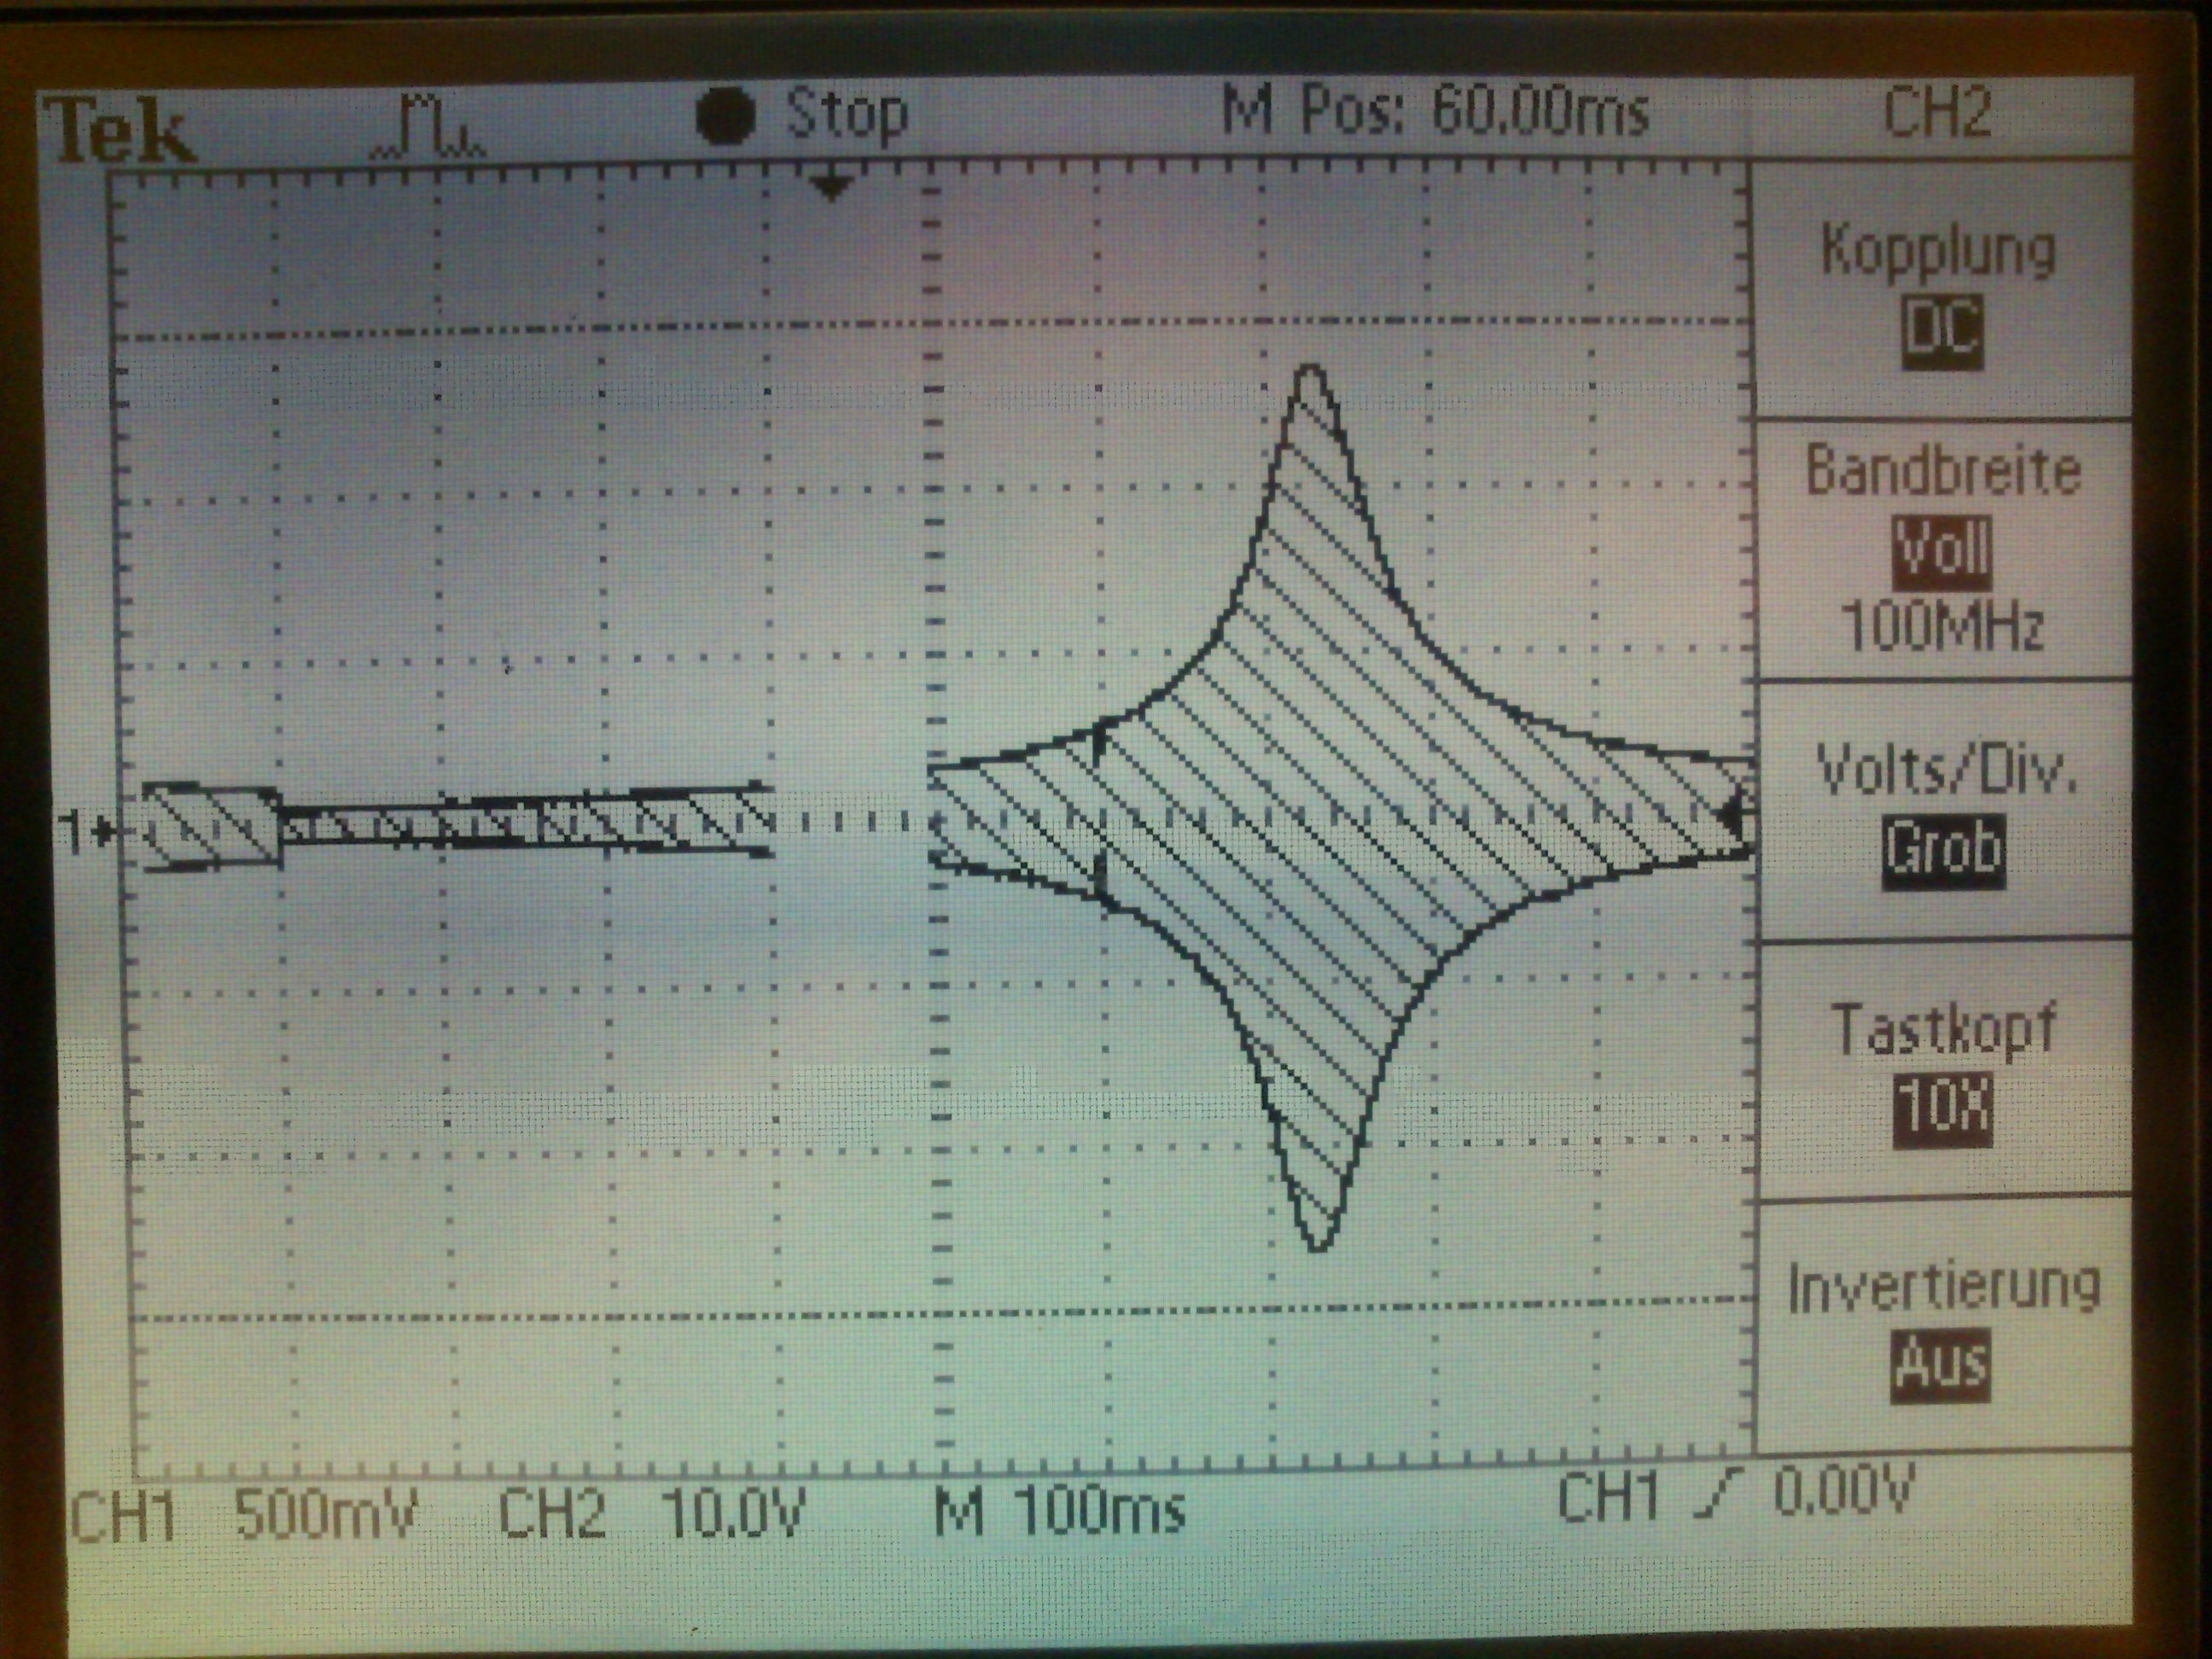
\includegraphics[width=\linewidth]{versuch4/oszi/DSC_0397.JPG}
	\caption{Sweep-Messung}
\end{figure}
Die Verschiebung der Resonanzfrequenz gegenüber den vorigen Werten rührt wahrscheinlich daher, dass ich zwischenzeitlich den Versuch abbrechen musste, und ihn dann in der nächsten Woche fortgesetzt habe. Die neue Resonanzfrequenz betrug 525 kHz.

\subsubsection{Fourieranalysator}
Hier eine Tabelle der ermittelten Fourierkomponenten:\\
\begin{tabular}{|l|l|l|}
	\hline
	Frequenz & Amplitude & Kommentar\\
	\hline
	\hline
	175 kHz & 1.32/2 V & 1/3 der maximalen Amplitude\\
	\hline
	105 kHz & 800/2 mV & 1/5 der maximalen Amplitude\\
	\hline
	75 kHz & 640/2 mV & knapp über 1/7 der maximalen Amplitude\\
	\hline
	58.33 kHz & 520/2 mV & knapp über 1/9 der maximalen Amplitude\\
	\hline
\end{tabular}

Als nächstes wurde der Schwingkreis mit einem Rechtecksignal von 10 kHz angesteuert. Dabei ergab sich folgendes Bild:
\begin{figure}[H]
	\centering
	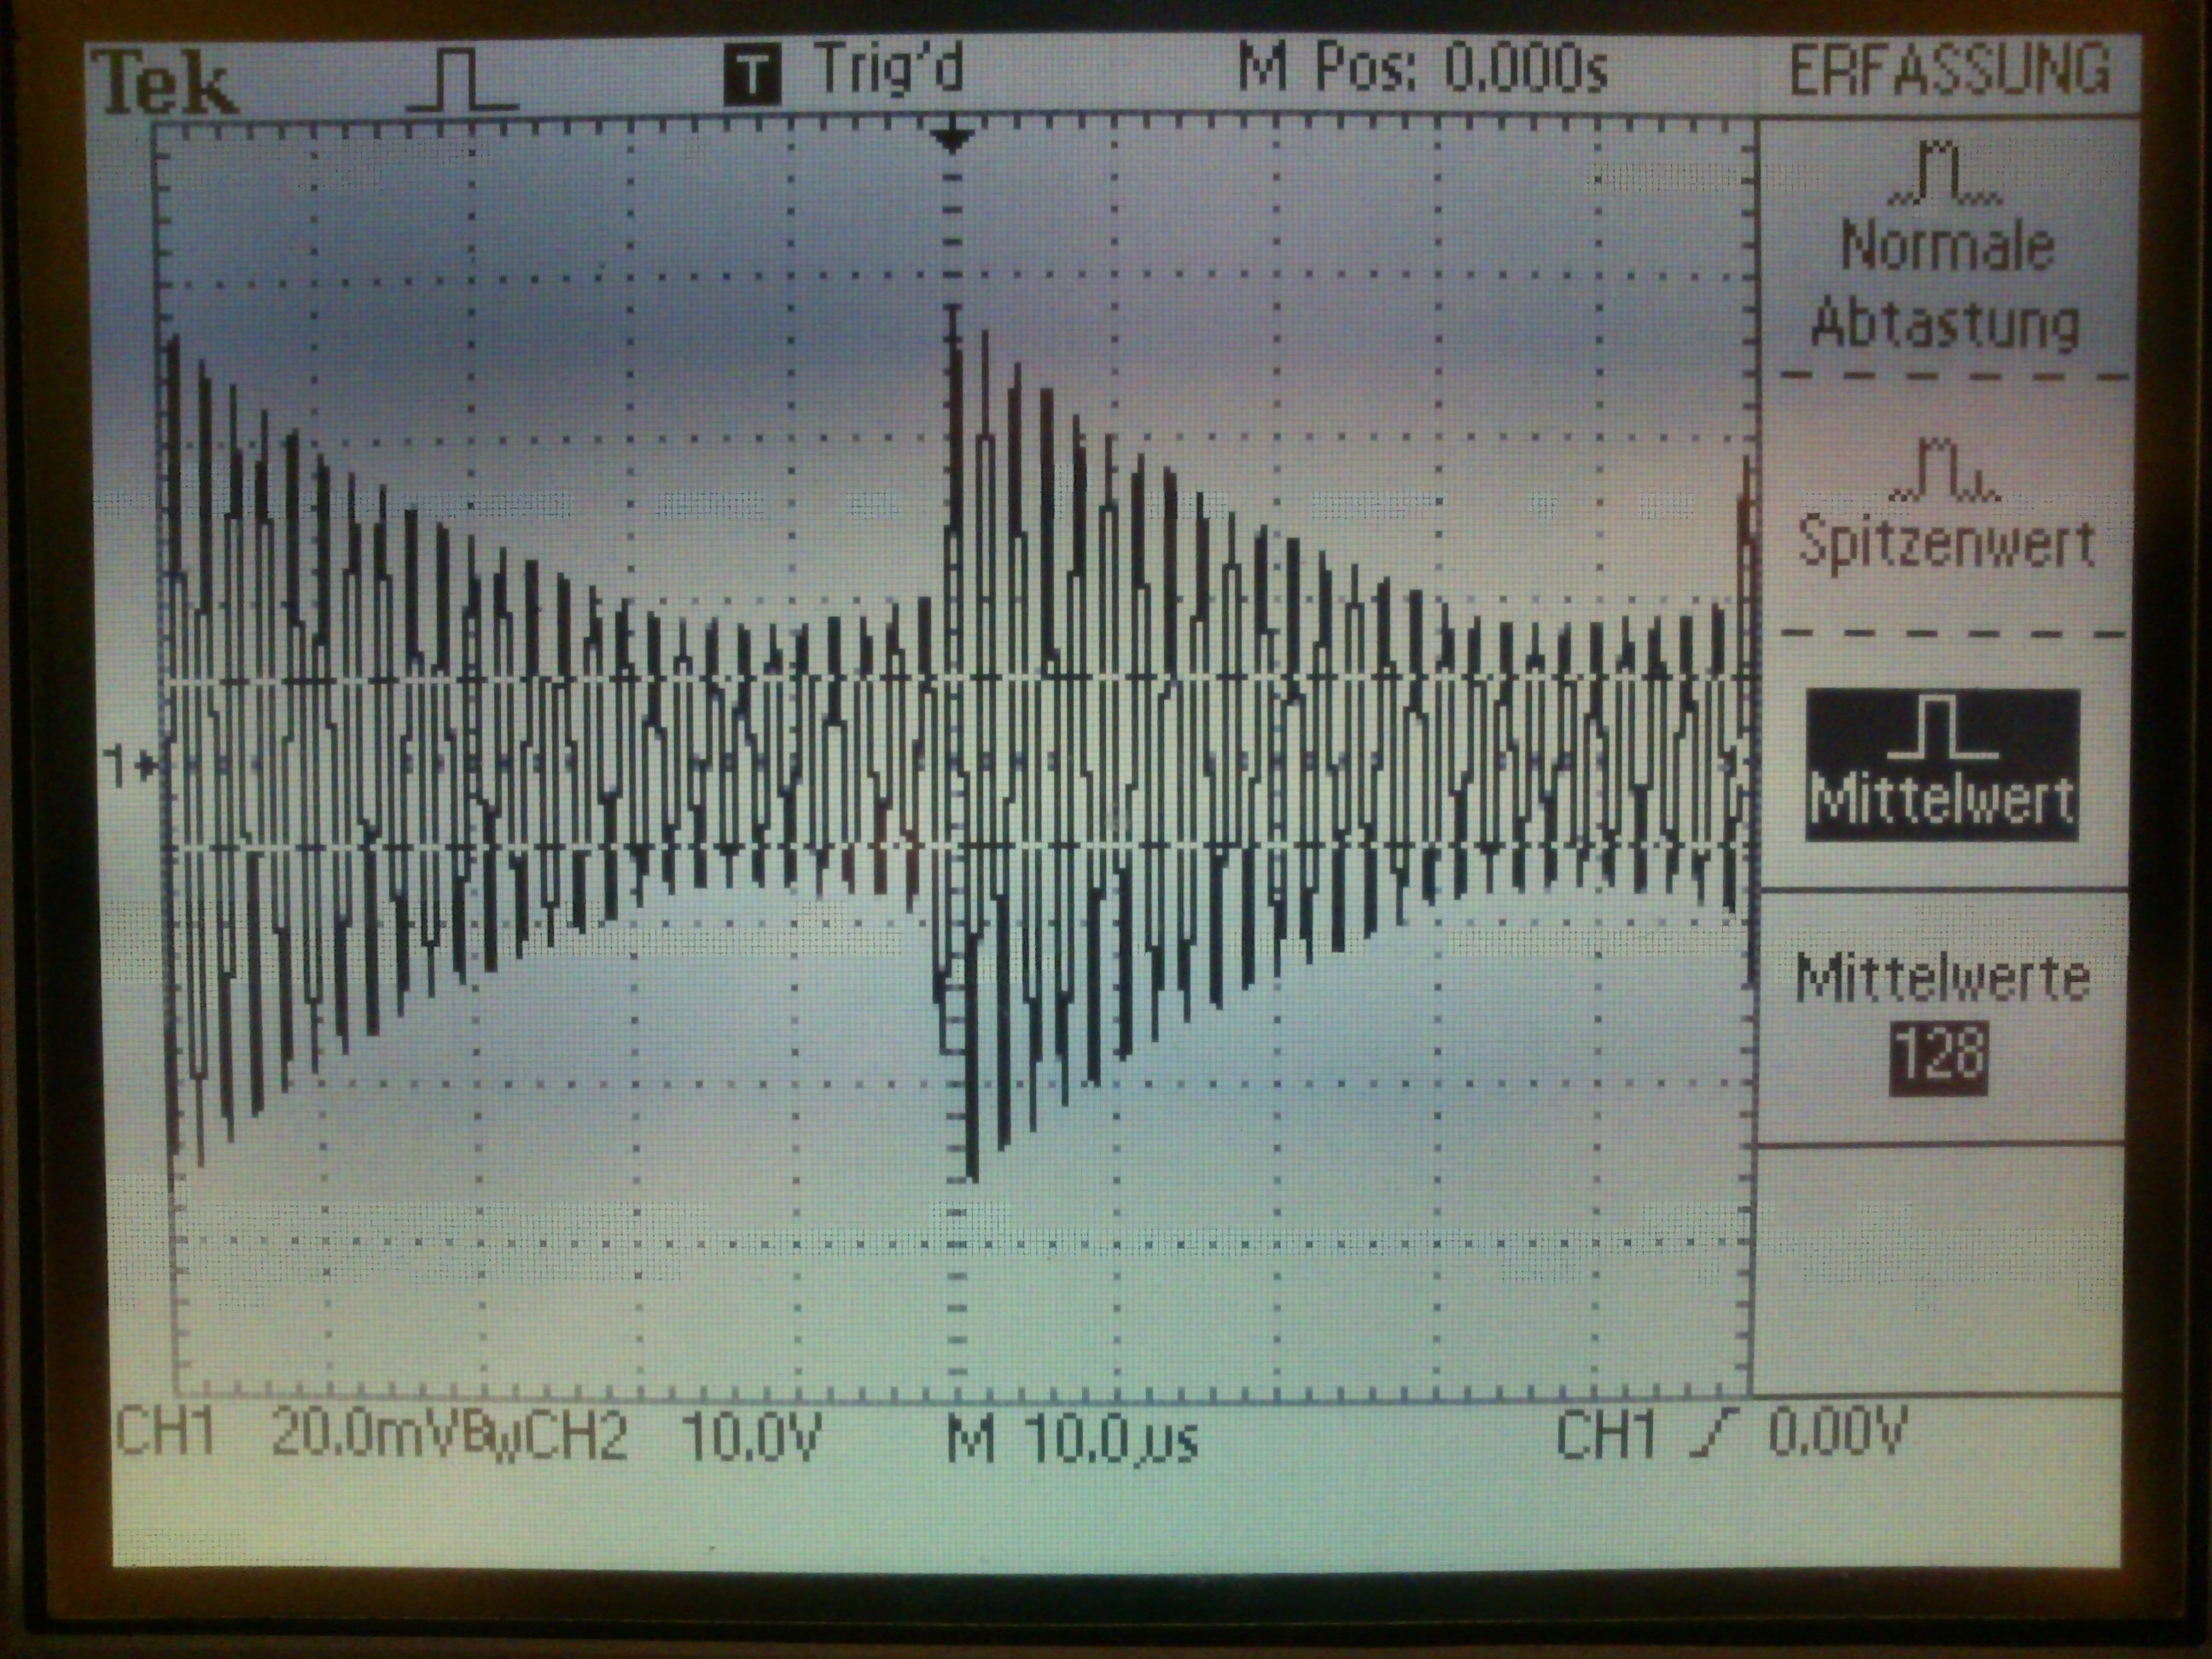
\includegraphics[width=\linewidth]{versuch4/oszi/DSC_0411.JPG}
	\caption{Reaktion des Schwingkreises auf eine Steigende Flanke}
\end{figure}
Man erkennt, dass 26 Schwingungen innerhalb von 50 \mu s stattfinden, daraus folgt eine Frequenz von 0.4 MHz.

\subsection{FFT}
Die erste Spektrallinie wurde zu 1kHz, 63,2 dB bestimmt.
\begin{figure}[H]
	\centering
	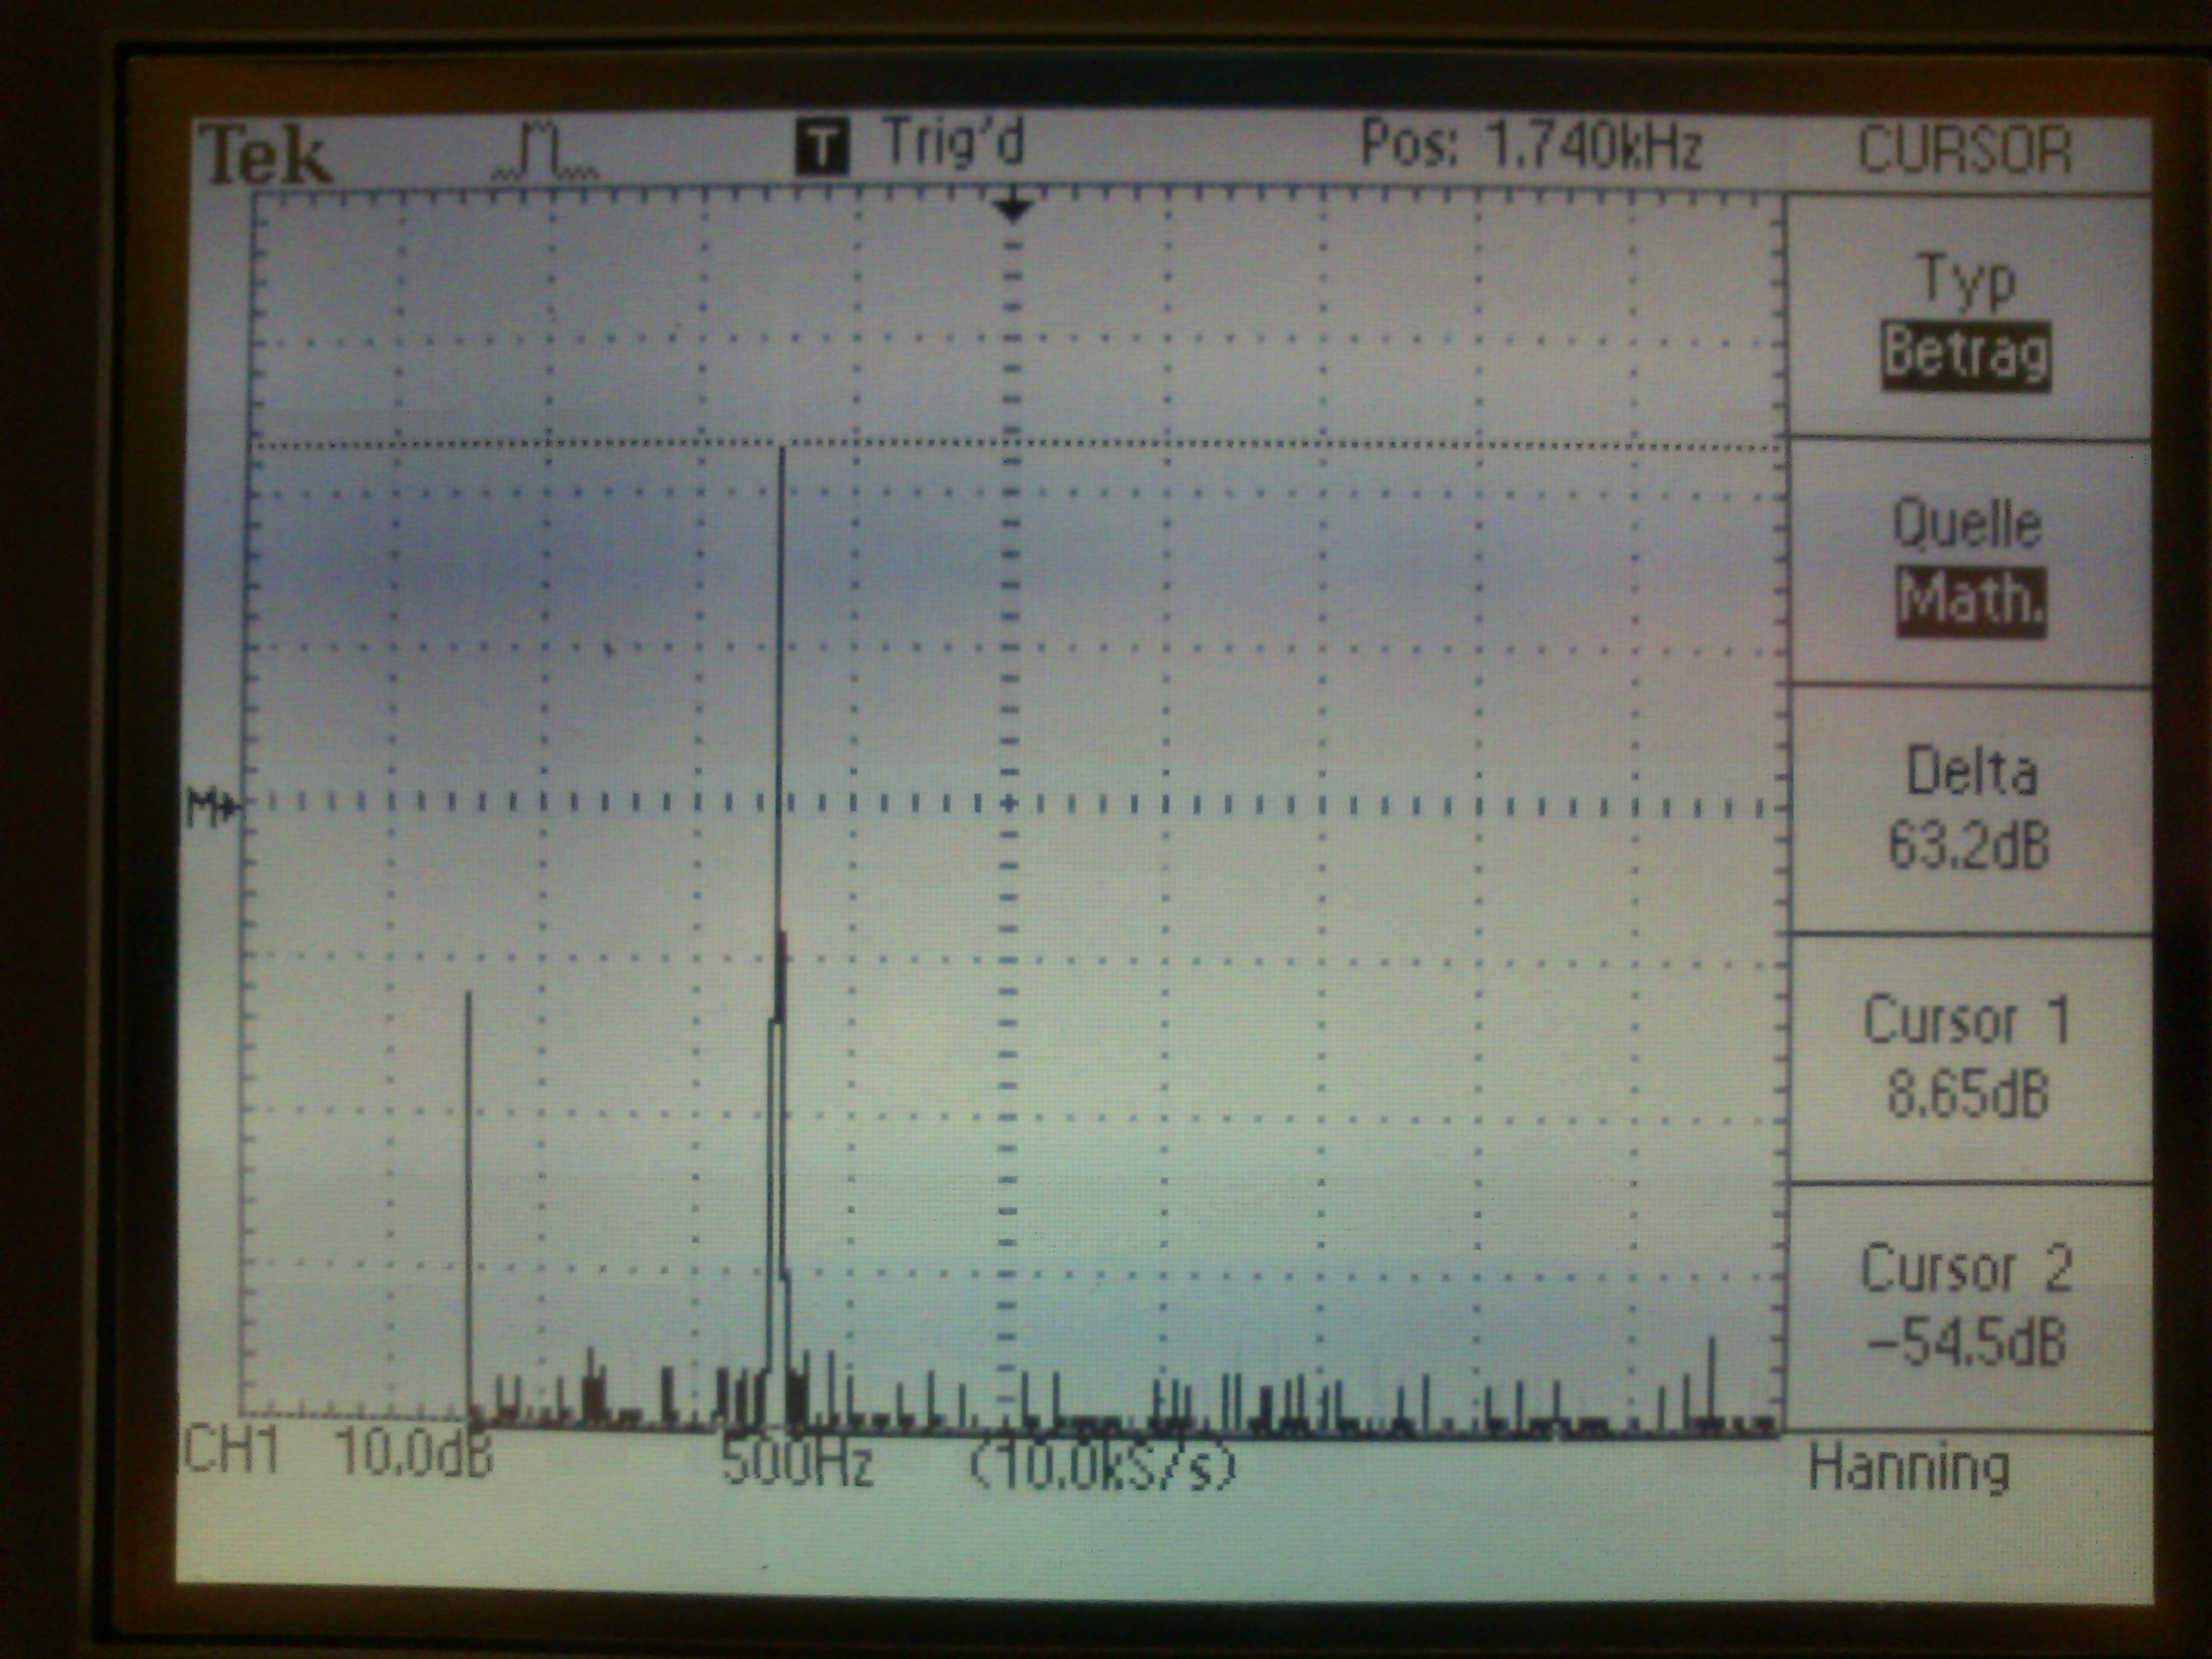
\includegraphics[width=\linewidth]{versuch4/oszi/DSC_0416.JPG}
	\caption{Bestimmung der Spektrallinien}
\end{figure}
Da die restlichen Spektrallinien nicht mehr über das Quantisierungsrauschen hinaustraten, haben ich den Signalgenerator auf Rechteck gestellt, damit traten deutlich erkennbare Harmonische auf:\\\\
\begin{tabular}{|l|l|l|}
	\hline
	Frequenz & Dämpfung & Amplitude\\
	\hline
	\hline
	3 kHz & 1,58 dB & 4,8 V = $U_1$\\
	\hline
	5 kHz & -3,75 dB & 2,6 V = $U_2$\\
	\hline
	7 kHz & -5,75 dB & 2.06 V = $U_3$\\
	\hline
	9 kHz & -7,35 dB & 1.7 V = $U_4$\\
	\hline
	11 kHz & -9,35 dB & 1.36 V = $U_5$\\
	\hline
\end{tabular}
\vspace{0.3cm}

Der Klirrfaktor ergab sich somit zu:\\
$ \frac{\sqrt{\sum_{k=1}^3U_K^2}}{\sqrt{\sum_{k=0}^3U_K^2}} =  0.82479 $


Dann wurde der Signalgenerator auf Dreieck gestellt:
\begin{figure}[H]
	\centering
	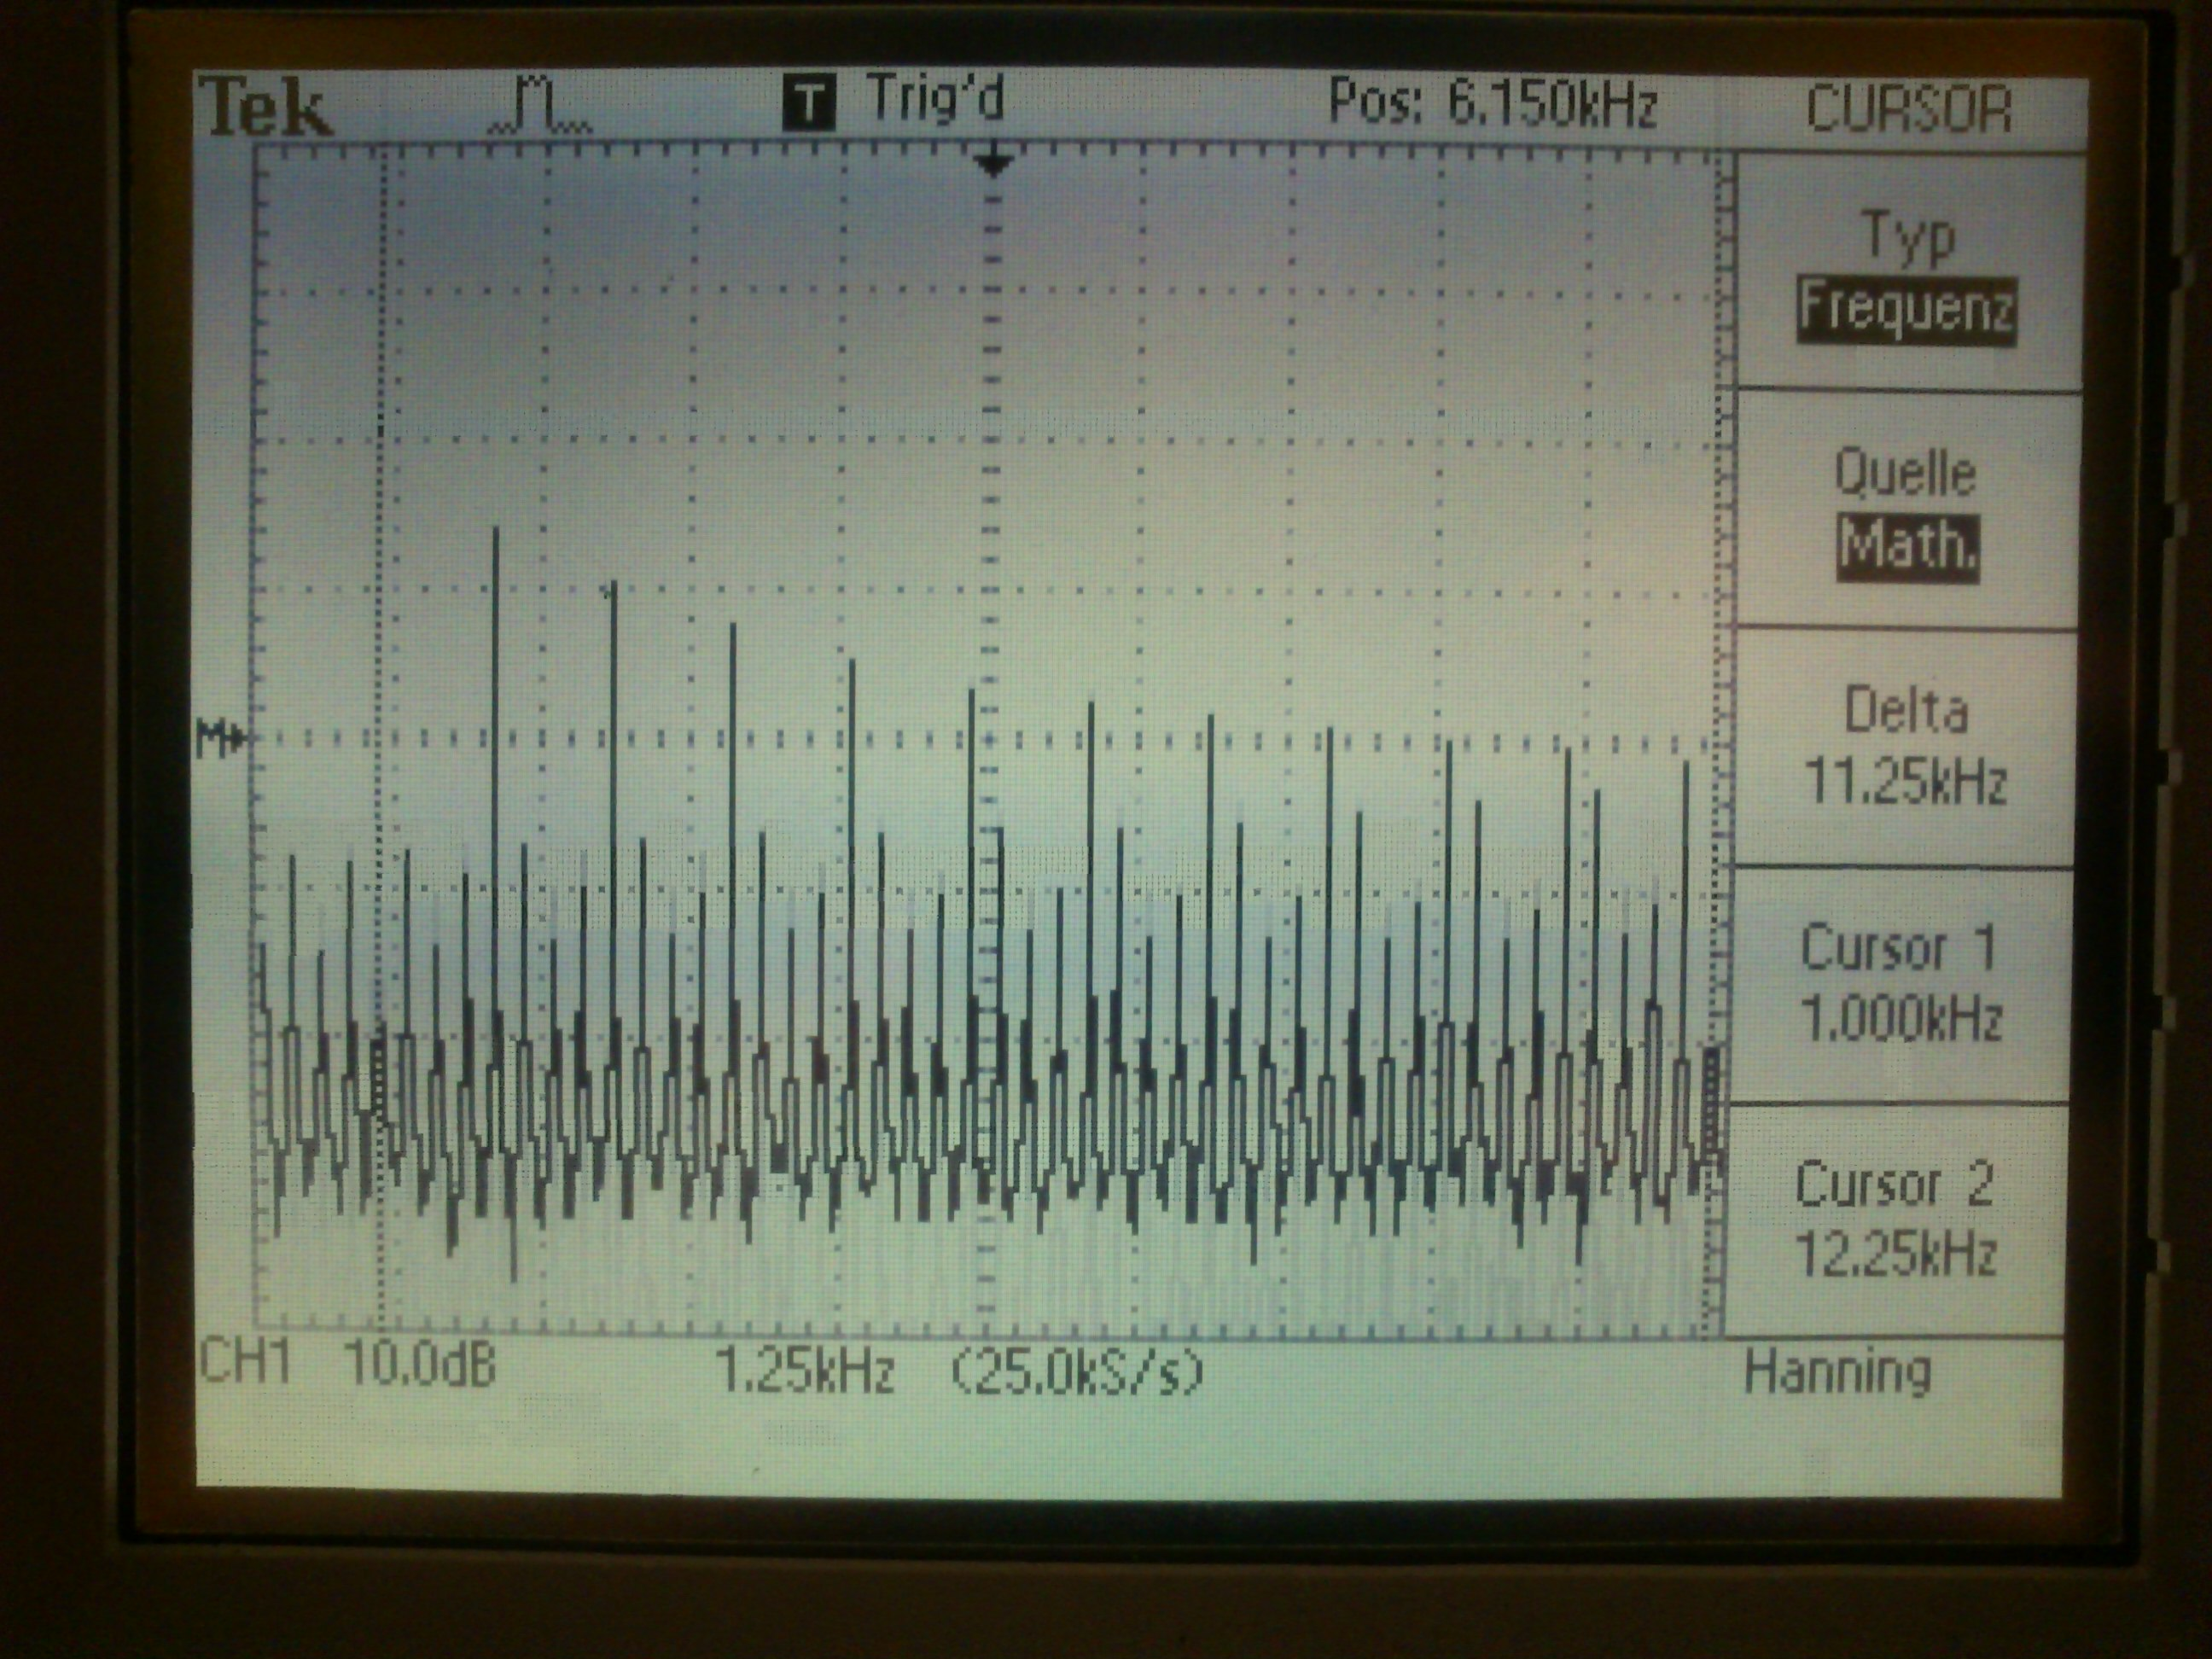
\includegraphics[width=\linewidth]{versuch4/oszi/DSC_0431.JPG}
	\caption{Spektrum des Dreieckssignals}
\end{figure}

%}}}

